\documentclass[12pt,a4paper]{article}
\usepackage{amsmath}

% Bibliografía %
\usepackage[backend=biber]{biblatex}
\addbibresource{referencias.bib} %Imports bibliography file
\usepackage[nottoc,numbib]{tocbibind}

\usepackage{vmargin}
\setpapersize{A4}
\setmargins{2.5cm}       % margen izquierdo
{1.5cm}                        % margen superior
{16.5cm}                      % anchura del texto
{23.42cm}                    % altura del texto
{10pt}                           % altura de los encabezados
{1cm}                           % espacio entre el texto y los encabezados
{0pt}                             % altura del pie de página
{2cm}                           % espacio entre el texto y el pie de página


\usepackage{amsfonts}
\usepackage{amssymb}
\usepackage[spanish]{babel}
\usepackage{csquotes}
% Rename "Cuadro" to "Tabla"
\addto\captionsspanish{\renewcommand{\tablename}{Tabla}}
\addto\captionsspanish{\renewcommand{\listtablename}{Índice de tablas}}

% Hyperrefs
\usepackage[hidelinks]{hyperref}

% Headers
\usepackage{fancyhdr}
\pagestyle{fancy}
\usepackage{cancel} 
\usepackage{graphicx}
\usepackage[dvipsnames,table]{xcolor}

% Figures
\usepackage{subcaption} % subfigures

% Tables
\usepackage{xltabular}
\newcolumntype{Y}{>{\centering\arraybackslash}X}
\usepackage{caption} % Para que las xltables salgan en la LOF 
\usepackage{hhline}

% Enumerates
\usepackage{enumitem}
\newcounter{Number} % i.e. Count inside tables
\newcommand{\countItem}{\stepcounter{Number}\theNumber.~}

% Todo notes
\usepackage{todonotes}


% Entorno de código - El argumento es para la referencia%
\usepackage{xparse,minted}
\newenvironment{code}[1]
{\small\snugshade\VerbatimEnvironment\begin{minted}[escapeinside=||,mathescape=true]{#1}}
{\end{minted}\endsnugshade} 

\newenvironment{code2}[1]
{\scriptsize\snugshade\VerbatimEnvironment\begin{minted}[escapeinside=||,mathescape=true]{#1}}
{\end{minted}\endsnugshade} 


\fancyhf{}
\cfoot[\thepage]{\thepage}
\lhead[\rightmark]{}
\rhead[]{\rightmark}
	
\usepackage{tocloft}

\renewcommand{\cftsubsecfont}{\normalfont\hypersetup{linkcolor=black}}
\renewcommand{\cftsubsubsecfont}{\normalfont\hypersetup{linkcolor=ForestGreen}}



\rhead{}
\lhead{\leftmark}
\cfoot{Página \thepage}
\renewcommand{\headrulewidth}{2pt}
\renewcommand{\footrulewidth}{1pt}


\begin{document}


\begin{titlepage}
\centering
{\includegraphics[width=0.4\textwidth]{escudo_umu_red_sq.png}\par}
\vspace{1cm}
{\bfseries\LARGE Universidad de Murcia \par}
\vspace{0.5cm}
{\scshape\Large Grado en Ingeniería Informática \par}
\vspace{0.5cm}
{\scshape\Large Compresión Multimedia \par}
{\scshape\Large Curso 22/23 \par}
\vspace{1cm}
{\scshape\Huge \textbf{Proyecto Final\\} \par}
\vspace{0.5cm}
{\scshape \Large Compresión de Imágenes Basada en DCT:\\Estudio Experimental \par}
\vspace{1.5cm}
\vfill


{ \Large\textbf{Javier Polo Gambín} \\
javier.polog@um.es\par}
\vspace{0.7cm}
{\textbf{Grupo: PCEO}\par}
\vspace{0.7cm}
\vfill
{\large Profesor: ???????? \par}
\vfill
{\Large \date{\today} \par}
\vfill
{\large \today \par}
\end{titlepage}

\newpage

\tableofcontents
\newpage 
\listoffigures

\setcounter{tocdepth}{2}

\newpage








\section{Resumen}
En el siguiente informe se expondrá el trabajo realizado como parte de las prácticas de la asignatura Compresión Multimedia.\\

En él se estudia 

(Veremos cómo funciona la compresión y cuáles son los factores que influyen en su eficacia. Además, presentaremos ejemplos prácticos de imágenes)


\newpage
\section{Introducción}
La compresión de imágenes desempeña un papel fundamental en diversos ámbitos, desde el campo de la tecnología y la ciencia hasta nuestra vida diaria. A lo largo de la historia, las imágenes han sido una herramienta poderosa para la comunicación y expresión cultural, la expresión artística y la transmisión de conocimiento. Desde las pinturas rupestres en la antigüedad hasta las imágenes científicas que revelan los misterios del universo o las publicaciones en redes sociales que consumimos a diario en nuestros teléfonos móviles, su impacto en la sociedad es innegable.\\

Con la era digital, la generación y el consumo de imágenes ha crecido exponencialmente. Se envían y reciben más imágenes que en ningún otro momento en la historia, y es aquí donde la compresión de imágenes se vuelve esencial para superar los nuevos desafíos como el almacenamiento y la transmisión eficiente de datos asociados a este consumo masivo. Imaginemos una situación en la que queremos enviar una fotografía de alta resolución a través de una conexión de internet limitada. Sin una técnica de compresión adecuada, la transferencia de esa imagen podría llevar mucho tiempo o incluso ser imposible. Supongamos ahora que un centro médico debe comunicar a otro los resultados de una prueba de resonancia magnética. Estas imágenes suelen tener un tamaño considerable debido a su alta resolución y detalles precisos, que resulta fundamental conservar. Es en casos como estos donde la compresión de imágenes juega un papel crucial al reducir significativamente el tamaño del archivo sin perder información esencial.\\

Con el desarrollo de la Teoría de la información???, las mejoras tecnológicas y la investigación en este campo se han desarrollado diversas técnicas de compresión que buscan cumplir los objetivos anteriores. En este estudio, utilizamos codificadores basados en la técnica de codificación Huffman. Esta técnica se basa en la utilización de un alfabeto de longitud variable, asignando códigos más cortos a los elementos que aparecen con mayor frecuencia. Al aplicar la codificación Huffman, se logra una reducción significativa en el tamaño de los archivos de imagen sin perder información esencial. La codificación Huffman ha demostrado ser una herramienta muy relevante en la compresión de imágenes. En el estudio experimental emplearemos dos variaciones de esta técnica \\

Además de la codificación Huffman, la transformada discreta del coseno (DCT) se ha convertido en un pilar fundamental en la compresión de imágenes. La DCT es una técnica que transforma la imagen del dominio espacial al dominio de frecuencia, lo que permite una representación más compacta de la imagen. Al aplicar la DCT, se logra una reducción de la redundancia espacial y se concentra la energía de la imagen en un conjunto selecto de coeficientes. Estos coeficientes se pueden cuantizar y codificar de manera eficiente, lo que contribuye a una compresión significativa sin comprometer demasiado la calidad visual.\\

En este estudio emplearemos ambas técnicas en conjunto para realizar una prueba experimental sobre una serie de imágenes seleccionadas. Estas experiencias nos permitirán valorar las capacidades y los límites de estas técnicas y determinar en qué casos debe usarse y de qué manera para que la compresión sea lo más efectiva posible.

??????? REVISAR ESTO ??????????



\newpage
\section{Metodología}
La codificación Huffman se basa en la asignación de códigos de longitud variable a los elementos en función de su frecuencia, de forma que emplea un alfabeto de longitud variable. Al utilizar esta codificación, los elementos que aparecen con mayor frecuencia se representan mediante códigos más cortos, mientras que a aquellos menos frecuentes se le asignan códigos más largos. Esta asignación se realiza de manera que no se produzcan ambigüedades en la decodificación de los datos comprimidos. De esta forma, se logra una compresión efectiva al aprovechar las repeticiones y patrones presentes en los datos originales.\\

Para la construcción del alfabeto de longitud variable pueden emplearse diversas tablas. En nuestro caso emplearemos 2 diferentes:
\begin{itemize}
    \item Tablas Huffman estándar, determinadas en base a observaciones empíricas?? \todo{Revisar}, y que se aplican sin variaciones, independientemente de la imagen particular.
    \item Tablas Huffman customizadas \todo{??}, que varían en función de cada imagen, atendiendo a la frecuencia de sus elementos.
\end{itemize}

Estas dos tablas en la codificación darán lugar a dos pares de compresor-descompresor. A partir de las tablas Huffman estándar desarrollaremos el compresor-descompresor \textbf{\textit{default}} y a partir de las customizadas el compresor-descompresor \textbf{\textit{custom}}.\\
\todo[inline]{Más info sobre Huffman/la DCT e indicar que es COMPRESIÓN CON PÉRDIDAS}

\subsection{Imágenes seleccionadas}
La selección de imágenes para el experimento se ha llevado a cabo de manera deliberada, basándome en el principio de diversidad y el potencial de análisis. Con este enfoque, se han elegido cuidadosamente imágenes que abarcan una amplia gama de características, como tamaño, composición, número de elementos, patrones y colores. El objetivo de esta selección es obtener ejemplos representativos que permitan apreciar las características fundamentales de los compresores utilizados y comprender las condiciones en las que su desempeño es mejor y peor.\\

Todas las imágenes son en formato \textit{BMP} por tratarse de un formato sin pérdidas (no podríamos concluir nada de un formato comprimido con pérdidas, como \textit{jpeg}, porque se estarían comparando las diferencias relativas de dos compresiones consecutivas pero no la compresión del fichero original). En el caso de las imágenes de fuente propia, las he obtenido realizando una captura de pantalla, lo que me permite almacenar el mapa de bits en el formato deseado (en oposición de imágenes descargadas de internet, de las que no puedo asegurar si se encuentran en su formato original o proceden de una conversión desde un formato con pérdidas). Todas las imágenes son de fuente propia salvo que se especifique lo contrario.\\

Los ficheros de las distintas imágenes pueden encontrarse en el directorio \textit{\textbackslash source\textbackslash Images\textbackslash original}.

\subsubsection{candados}
Esta imagen la he obtenido del material proporcionado por los profesores de la asignatura en el aula virtual para las prácticas de la asignatura. La he seleccionado debido a su abundancia de elementos detallados, ya que considero que esto permitirá apreciar las diferencias en el nivel de detalles preservados por cada tipo de compresor y factor de calidad. Además, gran parte de la imagen presenta tonos similares, principalmente tonos dorados, los cuales podrían ser aprovechados por el compresor para reducir el tamaño de la imagen.\\

La imagen es de $480x640$ píxeles y ocupa 900KB.\\

\begin{figure}[H]
    \centering
    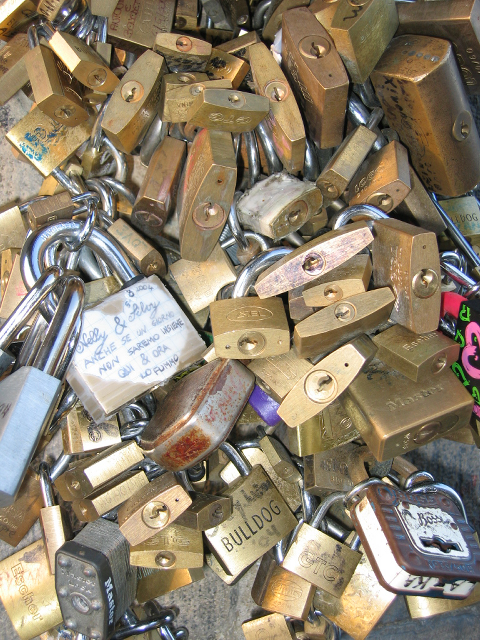
\includegraphics[scale=0.4]{images/candados.png}
    \caption{candados.bmp}
    
\end{figure}

\subsubsection{lennon}
He seleccionado esta imagen debido a su fondo uniforme, lo cual permitirá al compresor aprovecharlo y lograr un buen ratio de compresión. Además, la imagen contiene elementos detallados, como las gafas y el micrófono, que resultará interesante analizar en términos de cómo conservan sus detalles en diferentes configuraciones de los compresores.\\

La imagen es de $1375x1031$ píxeles y ocupa 4.05MB. Se trata de una imagen bastante grande, puesto que creo que resultará interesante extraer datos sobre el desempeño de los compresores en imágenes de distintos tamaños (grandes y pequeños).\\

\begin{figure}[H]
    \centering
    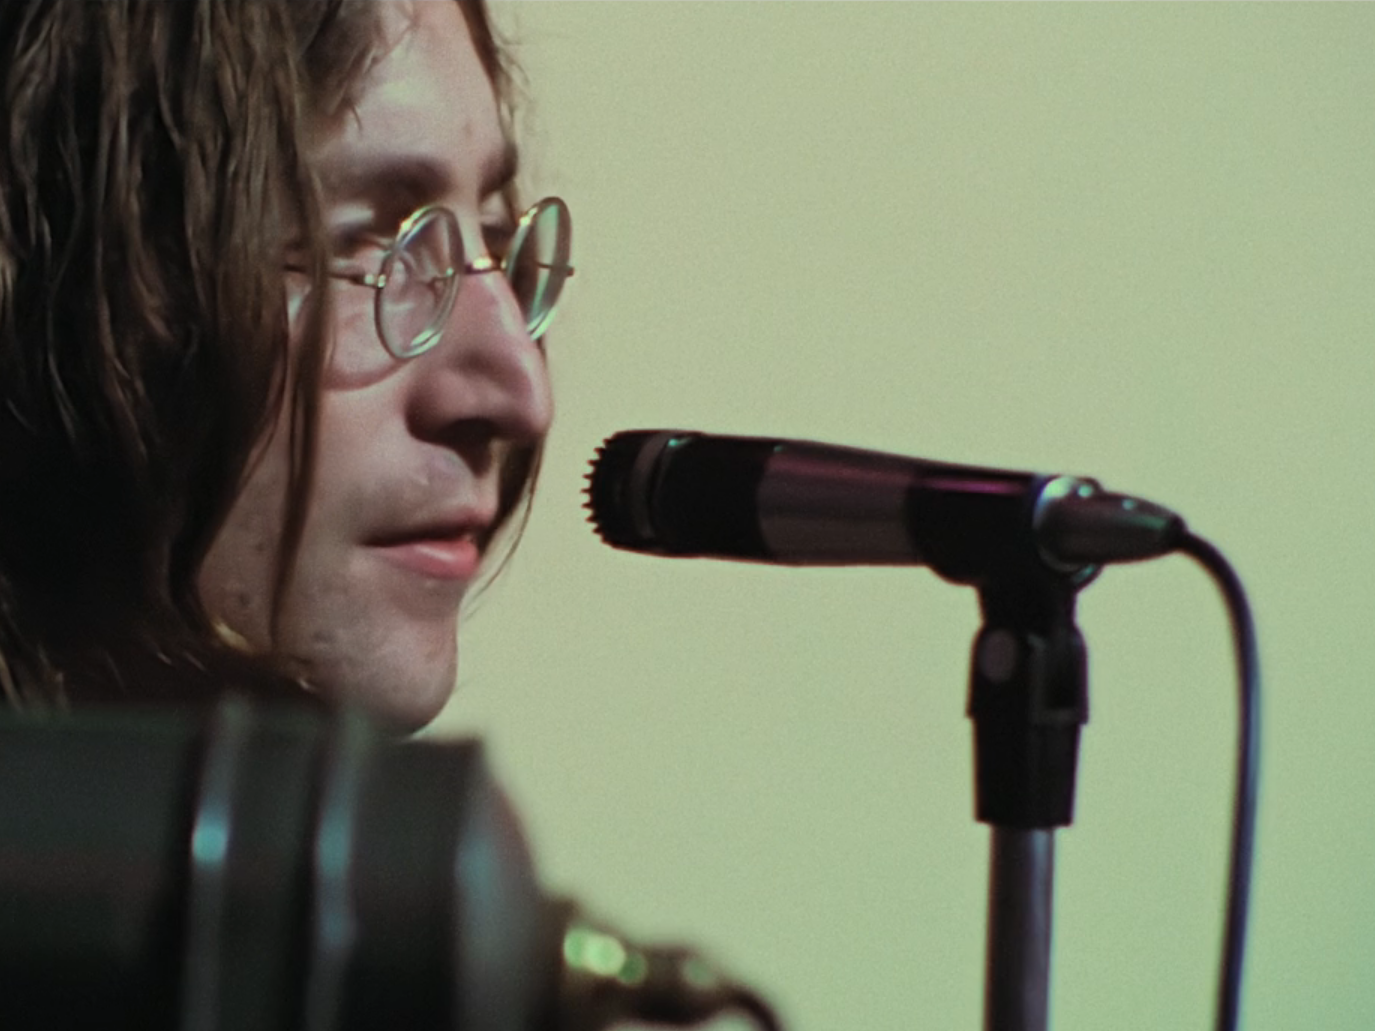
\includegraphics[scale=0.2]{images/lennon.png}
    \caption{lennon.bmp}
    
\end{figure}

\subsubsection{graph}
Esta imagen representa una gráfica en 3 dimensiones generada en Matlab. Considero que esta imagen es interesante debido a que el gráfico presenta regiones del mismo color, donde cada unidad de la cuadrícula tiene un color uniforme. Esto implica que existe una correlación que puede ser explotada por el compresor. Sin embargo, también observamos que las regiones adyacentes tienen colores similares, lo cual plantea la interrogante de cómo el compresor manejará estos casos, es decir, si las secciones se fusionarán o permanecerán bien delimitadas, entre otros aspectos a estudiar. Además, resulta relevante analizar si se mantiene la forma general de la gráfica o si en niveles de compresión más altos comienza a deformarse.

En base a esto, planteo la hipótesis de que esta imagen ofrecerá buenos resultados de compresión, debido al fondo blanco uniforme y a la correlación mencionada anteriormente. Sin embargo, no puedo realizar una estimación precisa sobre cómo se verán afectados los números o los propios ejes en niveles elevados de compresión.\\

La imagen es de $800x800$ píxeles y ocupa 1.83MB. Es por tanto, una imagen de tamaño mediano.\\

\begin{figure}[H]
    \centering
    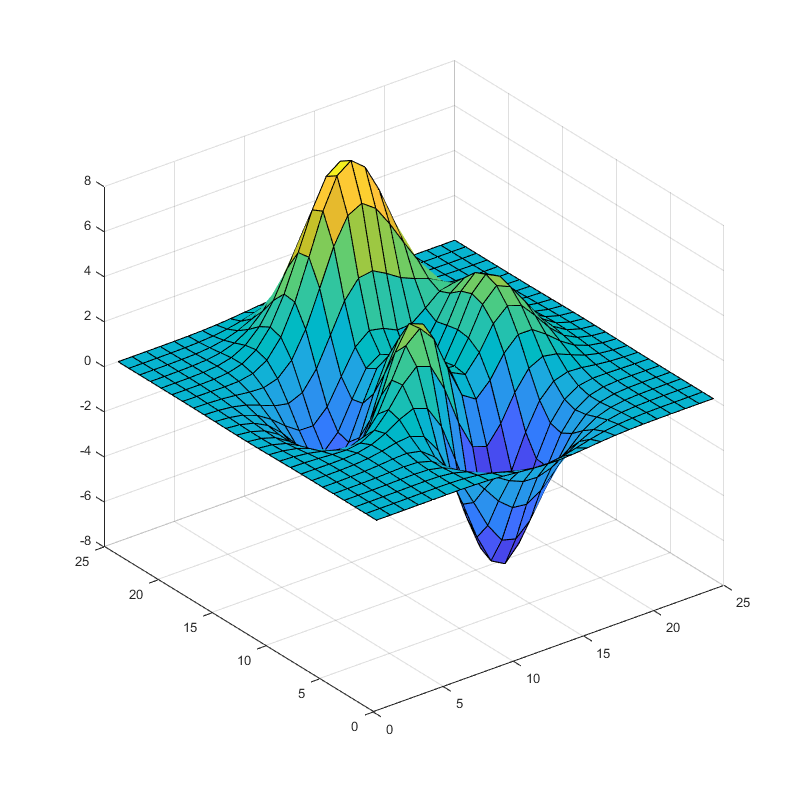
\includegraphics[scale=0.4]{images/graph.png}
    \caption{graph.bmp}
    
\end{figure}

\subsubsection{lena}
Esta imagen ha sido ampliamente utilizada en el campo de la compresión de imágenes como referencia para evaluar el desempeño de los algoritmos compresores. Es una elección interesante debido a las áreas con alto nivel de detalle, como el cabello y los ojos, y su fondo no uniforme pero relativamente plano. La hemos incluido en nuestro estudio debido a su relevancia histórica y por ser un estándar ampliamente reconocido en la industria.\\

Como hipótesis inicial, a pesar de ser una imagen en blanco y negro sin transiciones abruptas de color, considero que los resultados obtenidos no serán óptimos debido a la gran cantidad de detalles que contiene. Es probable que no sea posible alcanzar tasas de compresión elevadas sin perder una considerable cantidad de información visual.\\

La imagen es de $512x512$ píxeles y ocupa 768KB.\\

\begin{figure}[H]
    \centering
    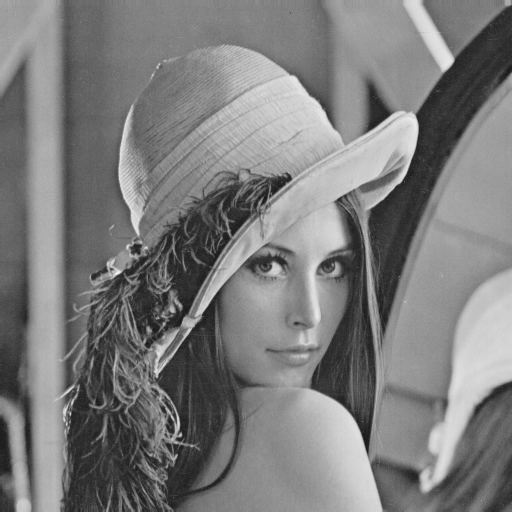
\includegraphics[scale = 0.5]{images/lena.png}
    \caption{lena.bmp}
    
\end{figure}

\subsubsection{mandrill}

\subsubsection{noise} \label{noisepre}
Esta imagen ha sido generada utilizando un sencillo programa en Python, donde los píxeles de colores se han asignado de manera aleatoria. En este caso, se espera que los resultados de la compresión sean muy deficientes, ya que los compresores aprovechan la correlación espacial para lograr una mayor compresión. Sin embargo, en esta imagen, dicha correlación es prácticamente inexistente, lo que implica que para mantener la similitud visual, se requerirán prácticamente todos los coeficientes de la transformada de coseno discreta (DCT), lo que resultará en tasas de compresión extremadamente bajas.\\

El objetivo de incluir esta imagen es evaluar el rendimiento de cada compresor ante un caso altamente desfavorable. Posteriormente, se compararán estos resultados con los obtenidos en un caso favorable, con el fin de destacar la importancia de la correlación espacial en el rendimiento de estos compresores.\\

La imagen es de $320x240$ píxeles y ocupa 225KB.\\

\begin{figure}[H]
    \centering
    
\includegraphics[scale = 0.8]{images/noise.png}
    \caption{noise.bmp}
    
\end{figure}


\subsubsection{pattern}
En el caso de esta imagen, debido a su patrón repetitivo, se espera que la transformada de coseno discreta (DCT) pueda aprovechar la redundancia espacial presente en la imagen. Además, la codificación Huffman podría ser eficiente en la compresión de los elementos más repetitivos dentro del patrón. Con base en esta consideración, mi hipótesis es que esta imagen debería alcanzar altos niveles de compresión sin perder significativamente el parecido visual con la imagen original.\\

Será interesante realizar una comparación entre los resultados obtenidos en esta imagen y los de la imagen anterior que carecía de correlación espacial. Esto nos permitirá analizar y contrastar los efectos de la correlación espacial en los resultados de compresión (\ref{noisepre}).\\

La imagen es de $320x240$ píxeles y ocupa 225KB. La he escogido del mismo tamaño que la anterior para poder comparar ambas mejor.\\

\begin{figure}[H]
    \centering
    
\includegraphics[scale = 0.8]{images/pattern.png}
    \caption{pattern.bmp}
    
\end{figure}


\subsubsection{color\_bars}
Cuando una imagen contiene líneas verticales, estas líneas se traducen en coeficientes DCT con valores altos en las frecuencias verticales. En otras palabras, estas líneas generan energía concentrada en las componentes de alta frecuencia vertical de la imagen. Como resultado, muchos coeficientes en esas frecuencias tras realizar la DCT tendrán valores significativos, mientras que los coeficientes en otras frecuencias pueden tener valores cercanos a cero. Además, como solamente hay 8 líneas verticales anchas, los valores deberían concentrarse todavía más en algunos pocos componentes. De esta manera, durante la cuantización se podrá asignar a estos componentes etiquetas más pequeñas, para conseguir resultados de compresión muy buenos.\\

Mediante este ejemplo, busco evaluar un caso extremadamente favorable para los compresores. Se espera que esta imagen alcance las tasas de compresión más elevadas entre todas las que se están probando, con una diferencia visual prácticamente imperceptible en comparación con la imagen original para la mayoría de los factores de calidad evaluados\\  

La imagen es de $640x480$ píxeles y ocupa 900KB.\\
 
\begin{figure}[H]
    \centering
    
\includegraphics[scale=0.6]{images/color_bars.png}
    \caption{color\_bars.bmp}
    
\end{figure}

\subsubsection{explorer}
Esta imagen muestra un fragmento del explorador de archivos de Microsoft Windows 10, que contiene tanto texto como iconos. En nuestro análisis, nos enfocaremos en evaluar si el texto, los botones y otros elementos como los iconos se mantienen legibles y conservan un nivel adecuado de detalle.\\

Mediante este ejemplo, buscamos examinar el comportamiento de los compresores en una imagen que presenta texto sobre un fondo plano. Las diferencias visuales pueden tener un impacto significativo en la legibilidad del texto, por lo que resulta especialmente interesante estudiar cómo los compresores afectan a esta característica. Además, la imagen también contiene iconos pequeños, los cuales deseamos preservar con un alto nivel de detalle.\\

A primera vista, el fondo plano nos podría llevar a pensar que se obtendrán buenos resultados de compresión. Sin embargo, debido a la fuerte condición de que el texto debe ser legible, resulta difícil realizar una estimación precisa sobre los resultados obtenidos.\\

La imagen es de $720x320$ píxeles y ocupa 675KB.\\

\begin{figure}[H]
    \centering
    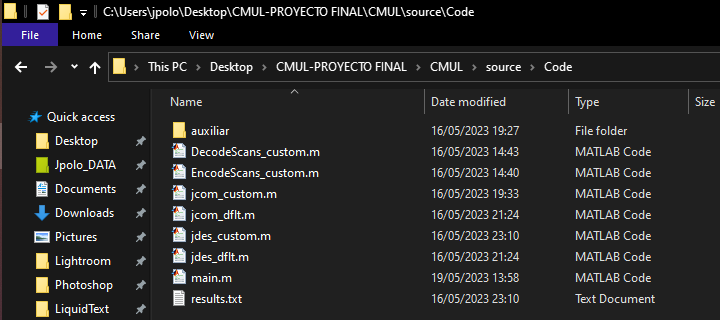
\includegraphics[scale=0.5]{images/explorer.png}
    \caption{explorer.bmp}
    
\end{figure}


\subsubsection{gradient}
En la imagen vemos una progresión de colores que se produce de forma suave y sin cambios bruscos entre zonas de distinto color.\\

Creo que esta característica es relevante e interesante, ya que se encuentra comúnmente en muchas fotografías del mundo real, como los tonos del cielo o los elementos grandes que presentan distintos tonos de color según la iluminación. En estas situaciones, los cambios de color se producen de manera gradual en lugar de brusca. Como hipótesis inicial, creo que se irán formando distintas regiones del mismo color, es decir, que los colores se ``unifiquen'' en diferentes regiones. Sin embargo, debido a que el cambio de color es suave, considero que se podrán obtener buenos resultados de compresión sin sacrificar calidad visual.\\ 

Mediante esta imagen, tenemos como objetivo analizar el fenómeno que ocurre al comprimir un patrón de gradación de color de forma aislada, sin la presencia de otros elementos en la imagen que puedan condicionar este análisis. Los resultados obtenidos en este análisis nos permitirán extrapolarlos posteriormente a otras imágenes que contengan regiones de color con características similares.\\

La imagen es de $300x300$ píxeles y ocupa 263KB.\\

\begin{figure}[H]
    \centering
    
\includegraphics{images/gradient.png}
    \caption{gradient.bmp}
    
\end{figure}

\subsubsection{color\_shapes}
En esta imagen, podemos observar grandes zonas que comparten el mismo color, separadas por fronteras diagonales. Considero que esta imagen resulta interesante para analizar el comportamiento de los compresores con respecto a las líneas diagonales que delimitan las diferentes regiones. Esto se debe a que, al eliminar las componentes menos significativas durante el proceso de transformada de coseno discreta (DCT), se puede perder detalle visual, lo que podría ocasionar que las líneas diagonales presenten una apariencia ``escalonada''.\\

Basado en esta consideración, planteo la hipótesis de que los cambios drásticos entre las regiones en la imagen provocarán una pérdida significativa de calidad visual en las líneas diagonales, incluso con factores de compresión bajos. En consecuencia, se espera que los resultados de la compresión no sean muy buenos en este caso.\\

La imagen es de $320x240$ píxeles y ocupa 225KB.\\

\begin{figure}[H]
    \centering
    
\includegraphics[scale=0.8]{images/cshapes.png}
    \caption{cshapes.bmp}
    
\end{figure}

\subsubsection{x-ray}

\subsection{Obtención de datos experimentales}
Para obtener los datos experimentales se procede de la siguiente manera:\\

Para cada imagen en formato BMP sin compresión, se realiza el proceso de compresión y posterior descompresión utilizando ambos compresores desarrollados, es decir, el compresor por defecto y el compresor customizado (\ref{}). Este proceso se repite para cada uno de los siguientes valores del parámetro de calidad considerados.\\
\begin{figure}[H]
    \centering
\[
\text{caliQ} = [5,25,50,100,175,250,500,1000]
\]
    \caption{Valores tomados por el parámetro de calidad en la experimentación (mayor valor indica menor calidad?????).}
    
\end{figure}
\todo[inline]{revisar la definición de caliQ}.

Esta metodología nos permite examinar y comparar las diferencias entre los dos compresores/descompresores en un amplio rango de resultados, abarcando desde aquellos con una pérdida mínima de calidad hasta aquellos con una pérdida significativa de calidad. En general, se espera que los ejemplos con una mayor pérdida de calidad alcancen las tasas de compresión más altas.\\

\subsection{Comparación cualitativa de los resultados}
Uno de los objetivos de este estudio es determinar las circunstancias en las que cada compresor de imagen resulta adecuado. Intuitivamente, consideraremos que el resultado es adecuado cuando presenta un alto grado de parecido visual en comparación con la imagen original. Aunque este criterio no es el único factor a tener en cuenta, como discutiremos más adelante, resulta fundamental para determinar el desempeño de un compresor como ``adecuado''. En última instancia, el objetivo es lograr la compresión de una imagen reduciendo su tamaño sin perder la menor cantidad posible de información.\\

Resulta evidente que no existe una manera exacta de comprobar el parecido visual entre dos imágenes percibido por un sujeto. Por lo tanto, en este estudio realizaremos un análisis observando los distintos resultados obtenidos para algunos factores de calidad seleccionados, y señalaremos el grado de parecido visual alcanzado.\\


\subsection{Comparación cuantitativa de los resultados} \label{metricasCuant}
En esta sección, calcularemos diferentes métricas para realizar un análisis cuantitativo de los resultados obtenidos. Las métricas que utilizaremos son las siguientes:\\
\textbf{Ratio de Compresión (\textit{RC})}: Compara el tamaño de la imagen comprimida respecto al tamaño de la imagen original. Se calcula utilizando la siguiente fórmula
\[
RC = \frac{T_{Original}-T_{Final}}{T_{Original}}
\]
\textbf{Signal-to-Noise-Ratio (\textit{SNR})}: Calcula el ratio entre la cantidad de información codificada en la señal y la cantidad de error (ruido) obtenido. Se utiliza la siguiente fórmula:
\[
\frac{\sum_i^n(x_i-y_i)^2}{n}
\]
\todo[inline]{Revisar estas definiciones y fórmulas y copiarlas del PDF. Ordenar en el orden en el que se devuelven en el programa.}
\textbf{Error cuadrático medio (\textit{MSE}, Mean Squared Error)}: Establece una métrica entre imágenes basada en las diferencias entre el valor de los píxeles individuales de las imágenes. Como mide la diferencia entre imágenes, en principio cuanto menor sea este valor, más similares serán las dos imágenes y viceversa, aunque no siempre es así. La fórmula utilizada es:
\[
SNR\text{(db)} = 10\cdot \text{log}_{10} \left( \frac{\sum x_i^2}{\sum(x_j-y_j)^2} \right)
\]

Estos valores se calcularán para cada imagen, utilizando diferentes valores del factor de calidad, y se aplicarán tanto al compresor estándar como al compresor customizado.  De esta manera podremos establecer una métrica de cuánto difiere cuantitativamente el resultado de cada método respecto a la imagen original, lo que nos proporcionará una manera empírica de comparar los resultados obtenidos mediante los dos métodos de compresión. Es decir, podremos comparar de manera cuantitativa los resultados de ambos compresores.\\

Es importante destacar que esta no es el único factor que ha de tenerse en cuenta cuando se evalúa el desempeño de un compresor de imágenes. También resulta fundamental evaluar el parecido visual percibido de las imágenes comprimidas respecto a las originales. Es bien sabido que dos imágenes pueden diferir cuantitativamente pero tener un gran parecido visual. En principio buscamos satisfacer ambas condiciones, y las fórmulas anteriores nos proporcionan una manera de realizar este análisis cuantitativo.


\subsection{Características técnicas del hardware}
Es importante indicar las características del hardware empleado para la ejecución de las pruebas experimentales, para permitir la reproducibilidad de los experimentos y porque los resultados pueden variar considerablemente en función de las prestaciones del hardware sobre el que se trabaja.\\

\todo[inline]{(CITAR AQUÍ lo de que pueden variar (final del documento de la práctica)??)}

En este caso, la ejecución de los experimentos la he realizado sobre un ordenador con procesador AMD Ryzen™ 7 2700X @ 3.7Ghz , con 16GB de RAM instalada.


\subsection{Características técnicas del software}
Por las mismas razones de antes se indican las versiones concretas del software empleado.\\

La implementación de los distintos compresores y descompresores la he realizado en lenguaje \textit{Matlab}. Para la ejecución de las pruebas y obtención de los datos he empleado el software \textit{Matlab R2018b}, sobre sistema operativo Microsoft Windows 10 Pro.  

\newpage
\section{Resultados experimentales}
En esta sección, analizaremos los resultados obtenidos a partir de los experimentos realizados. Comenzaremos con el estudio cualitativo, seguido del estudio cuantitativo. Esta secuencia se debe a que el estudio cualitativo implica una apreciación subjetiva, y dado que soy yo quien analiza los resultados, debemos evitar caer en el sesgo de confirmación.\todo{citar esto de alguna pag con la definición}.\\  

El estudio cualitativo se enfoca en el parecido visual entre las imágenes originales y las comprimidas. Evaluaré la preservación de los detalles, la legibilidad del texto, la calidad de los colores y la apariencia general de las imágenes. Realizaré una comparación y señalaré cualquier diferencia notable. Cabe destacar que este análisis está sujeto a la interpretación personal.\\

Posteriormente, realizaremos el estudio cuantitativo, el cual se basa en las métricas definidas en la sección \ref{metricasCuant}. Calcularemos el Ratio de Compresión (\textit{RC}), el Signal-to-Noise Ratio (\textit{SNR}) y el Error Cuadrático Medio (\textit{MSE}) para cada imagen y para ambos compresores utilizados. Estas métricas nos proporcionarán una medida cuantitativa del desempeño de los compresores y nos permitirán comparar los resultados obtenidos.\\

Es importante tener en cuenta que, aunque el análisis cuantitativo nos brinda información objetiva, no debemos descartar la importancia del análisis cualitativo. Ambos enfoques son complementarios y nos ayudarán a evaluar de manera integral los resultados obtenidos en nuestros experimentos.\\

\subsection{Estudio cualitativo}
Debido a la cantidad considerable de datos generados durante los experimentos, hemos realizado un análisis preliminar de los resultados y decidido focalizar nuestra discusión en los valores del parámetro de calidad $50$, $100$ y $250$. Estos valores representan niveles de compresión baja, media y alta, respectivamente. No obstante, en casos específicos donde sea relevante, también mencionaremos otros valores.\\

Consideramos que estos valores seleccionados proporcionan una visión representativa de los resultados obtenidos y nos permitirán analizar el impacto de la compresión en las imágenes.\\

Cabe destacar que el proceso de estudio cualitativo se realiza sobre los ficheros de las imágenes obtenidas. Aquí simplemente se muestran en un tamaño reducido con fines orientativos, recomendamos consultar los ficheros correspondientes.\\

Los ficheros de las imágenes resultantes se encuentran en \textit{\textbackslash source\textbackslash Images\textbackslash decoded\_dflt} en el caso de las imágenes del compresor por defecto, y en \textit{\textbackslash source\textbackslash Images\textbackslash decoded\_custom} en el caso del compresor customizado.

\subsubsection{candados}
Primero se muestra la imagen original para tener una referencia:
\begin{figure}[H]
    \centering
    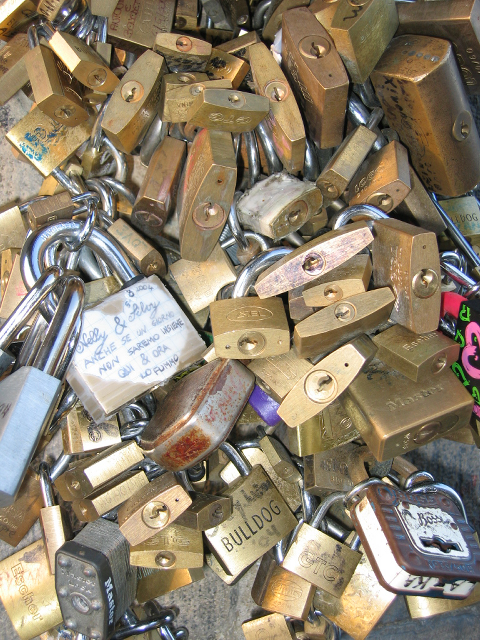
\includegraphics[width=0.20\textwidth]{images/candados.png}
    \caption[Referencia - candados]{Imagen original de referencia.}
    \label{fig:top_candados}
\end{figure}
    \vspace{0.5cm}

Imágenes resultantes:
\begin{figure}   [H]
    \begin{subfigure}{0.20\textwidth}
        \centering
        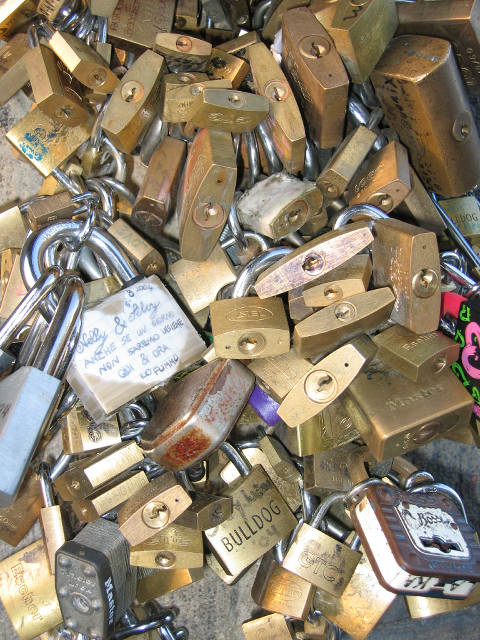
\includegraphics[width=\linewidth]{dflt/candados_Q50_dec_dflt.png}
        \caption{Default Q=50.}
        
    \end{subfigure}
    \hfill
    \begin{subfigure}{0.20\textwidth}
        \centering
        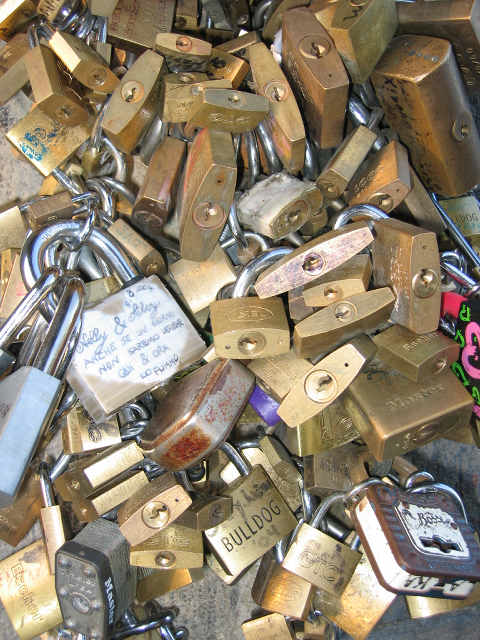
\includegraphics[width=\linewidth]{dflt/candados_Q100_dec_dflt.png}
        \caption{Default Q=100.}
        
    \end{subfigure}
    \hfill
    \begin{subfigure}{0.20\textwidth}
        \centering
        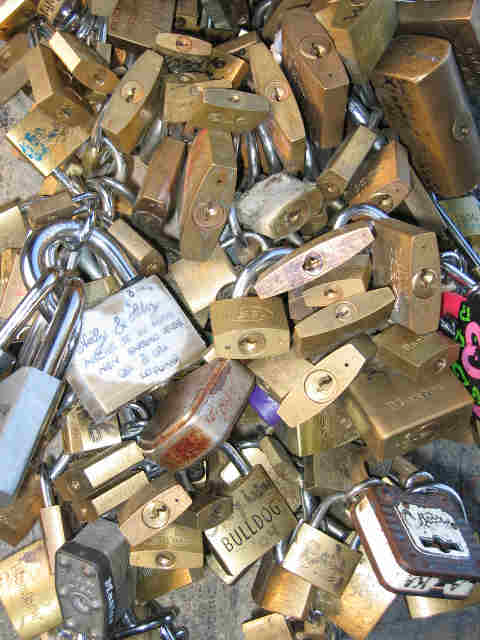
\includegraphics[width=\linewidth]{dflt/candados_Q250_dec_dflt.png}
        \caption{Default Q=250.}
        
    \end{subfigure}
    
    \vspace{0.5cm}
    
    \begin{subfigure}{0.20\textwidth}
        \centering
        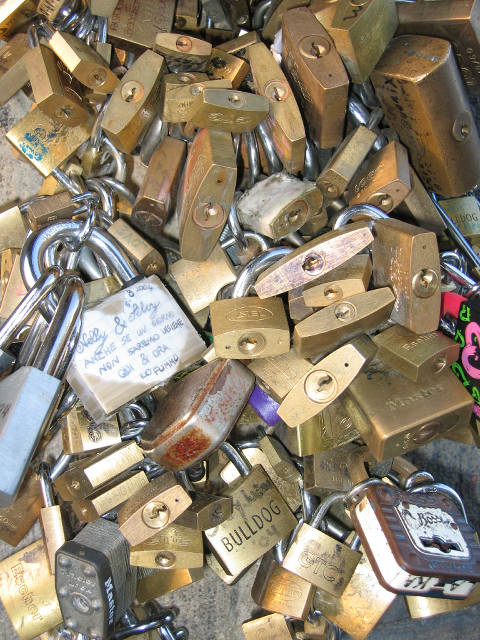
\includegraphics[width=\linewidth]{custom/candados_Q50_dec_custom.png}
        \caption{Custom Q=50.}
        
    \end{subfigure}
    \hfill
    \begin{subfigure}{0.20\textwidth}
        \centering
        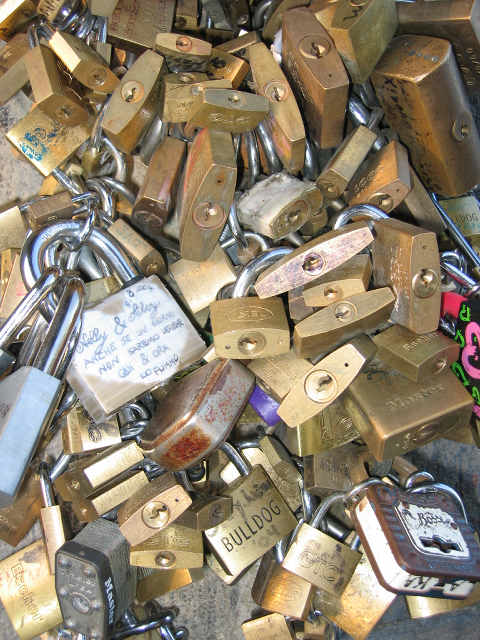
\includegraphics[width=\linewidth]{custom/candados_Q100_dec_custom.png}
        \caption{Custom Q=100.}
        
    \end{subfigure}
    \hfill
    \begin{subfigure}{0.20\textwidth}
        \centering
        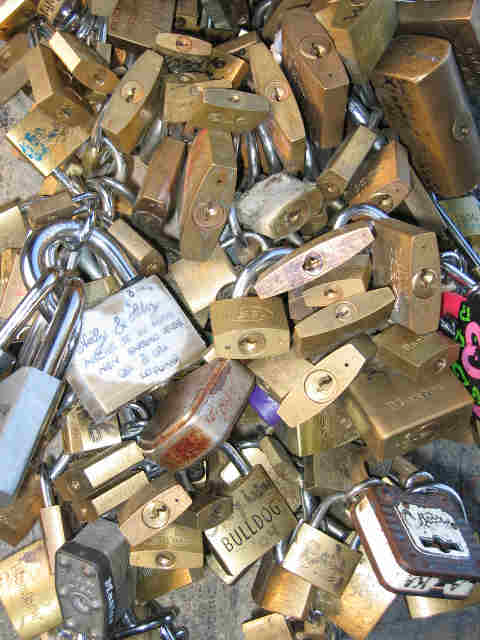
\includegraphics[width=\linewidth]{custom/candados_Q250_dec_custom.png}
        \caption{Custom Q=250.}
        
    \end{subfigure}
    
    \caption[Resultados experimentales - candado]{Resultados experimentales de la compresión de la imagen \textit{candados.bmp}.}
    \label{fig:candados_cuali}
\end{figure}

En la figura \ref{fig:top_candados}, vemos la imagen original que servirá de referencia. En la figura \ref{fig:candados_cuali} vemos las imágenes obtenidas como resultado de la compresión, en la primera fila por el compresor por defecto y en la segunda por el compresor customizado. Este formato será el mismo para el resto de imágenes.\\

Como observación inicial, podemos destacar un fenómeno interesante: Los resultados visuales para el compresor por defecto y el compresor customizado son prácticamente idénticos. Esto sucederá también con el resto de imágenes, de forma que se espera que la diferencia, si es que la hay, sea en el análisis cuantitativo.\\

Centrándonos en la imagen, con factor de calidad 50 no se aprecian diferencias muy significativas respecto a la original, como diferencia más notable se aprecia la textura de los candados, que empieza a verse más pixelada, así como los bordes de las marcas y las letras en las que se ve un efecto más pixelado. En cualquier caso estos detalles son muy sutiles.\\

Con factor de calidad 100 las diferencias anteriores se acentúan de forma moderada, y se ven claramente zonas en las que se forman ``manchas'' de píxeles. Esto es más notable en las zonas que no tienen un color uniforme. Las letras escritas sobre el candado grande (azul sobre fondo blanco) se distinguen pero con dificultad.\\

En el factor de calidad 250 las diferencias son enormes. La imagen adquiere una textura pixelada (se aprecian grandes bloques de píxeles que componen la imagen). Hay además fallos de color, porque aparecen colores y tonalidades donde antes parecía un color casi uniforme, y las letras no son distinguibles de ninguna manera. Consideramos que este resultado no es ya adecuado visualmente.\\

En este caso considero que el factor de calidad 100 es el más adecuado, puesto que aunque presenta más diferencias que el factor 50, la imagen se sigue viendo natural y los elementos como las letras continúan siendo visibles. El efecto de la pixelación todavía no es tan notable alterando bordes y colores y lo considero un resultado adecuado.\\



\subsubsection{lennon}
Primero se muestra la imagen original para tener una referencia:
\begin{figure}[H]
    \centering
    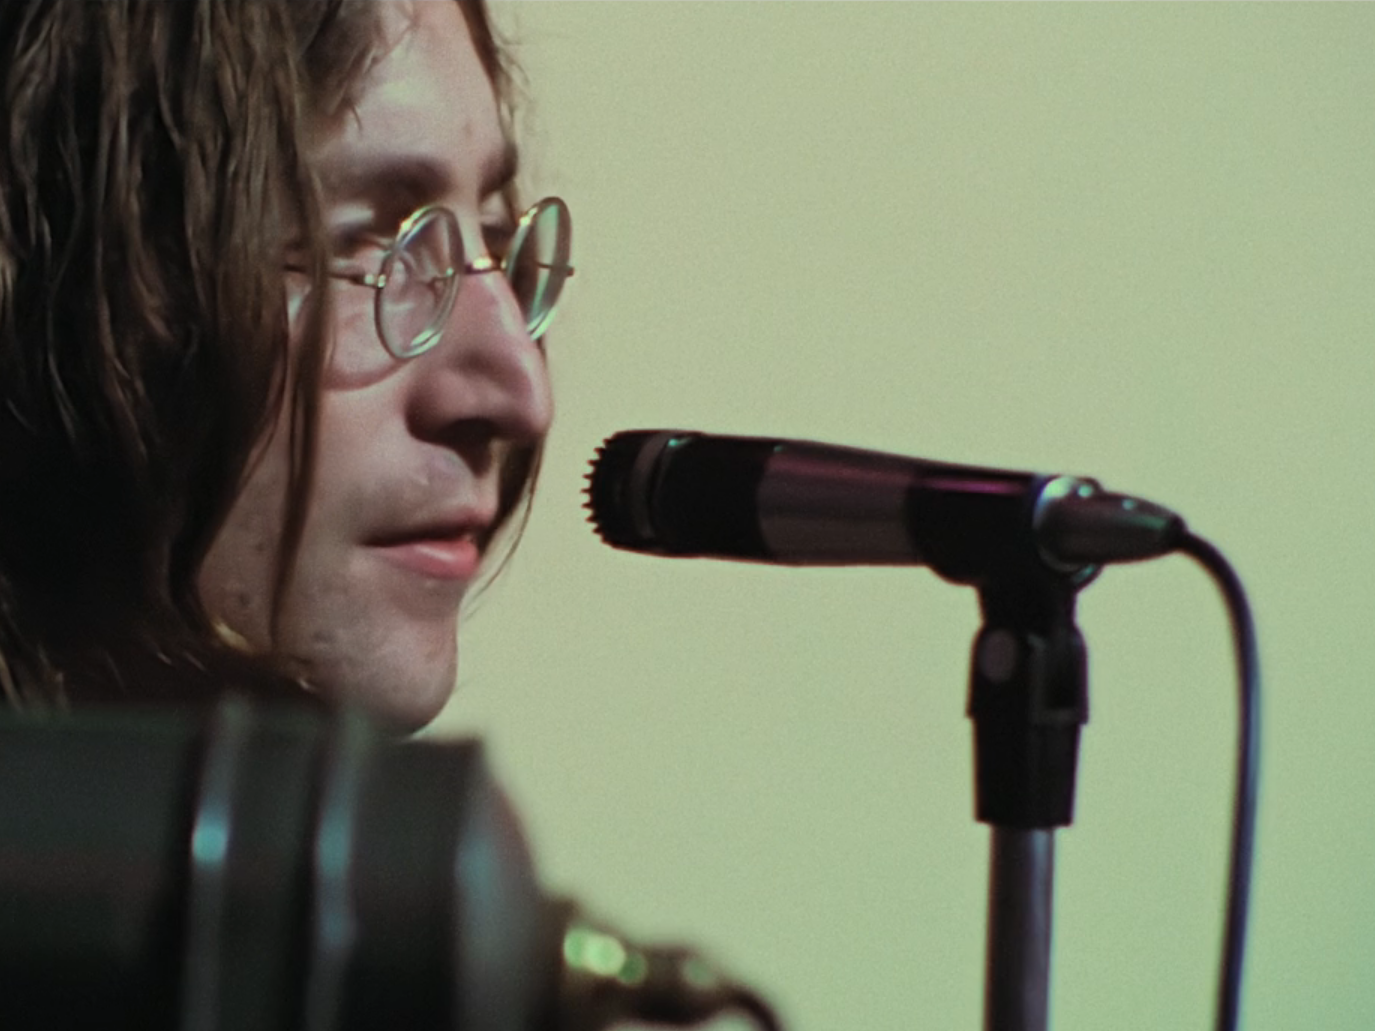
\includegraphics[width=0.30\textwidth]{images/lennon.png}
    \caption[Referencia - lennon]{Imagen original de referencia.}
    
 \end{figure}   
    \vspace{0.5cm}
    
Imágenes resultantes:
\begin{figure}   [H]   
    \begin{subfigure}{0.30\textwidth}
        \centering
        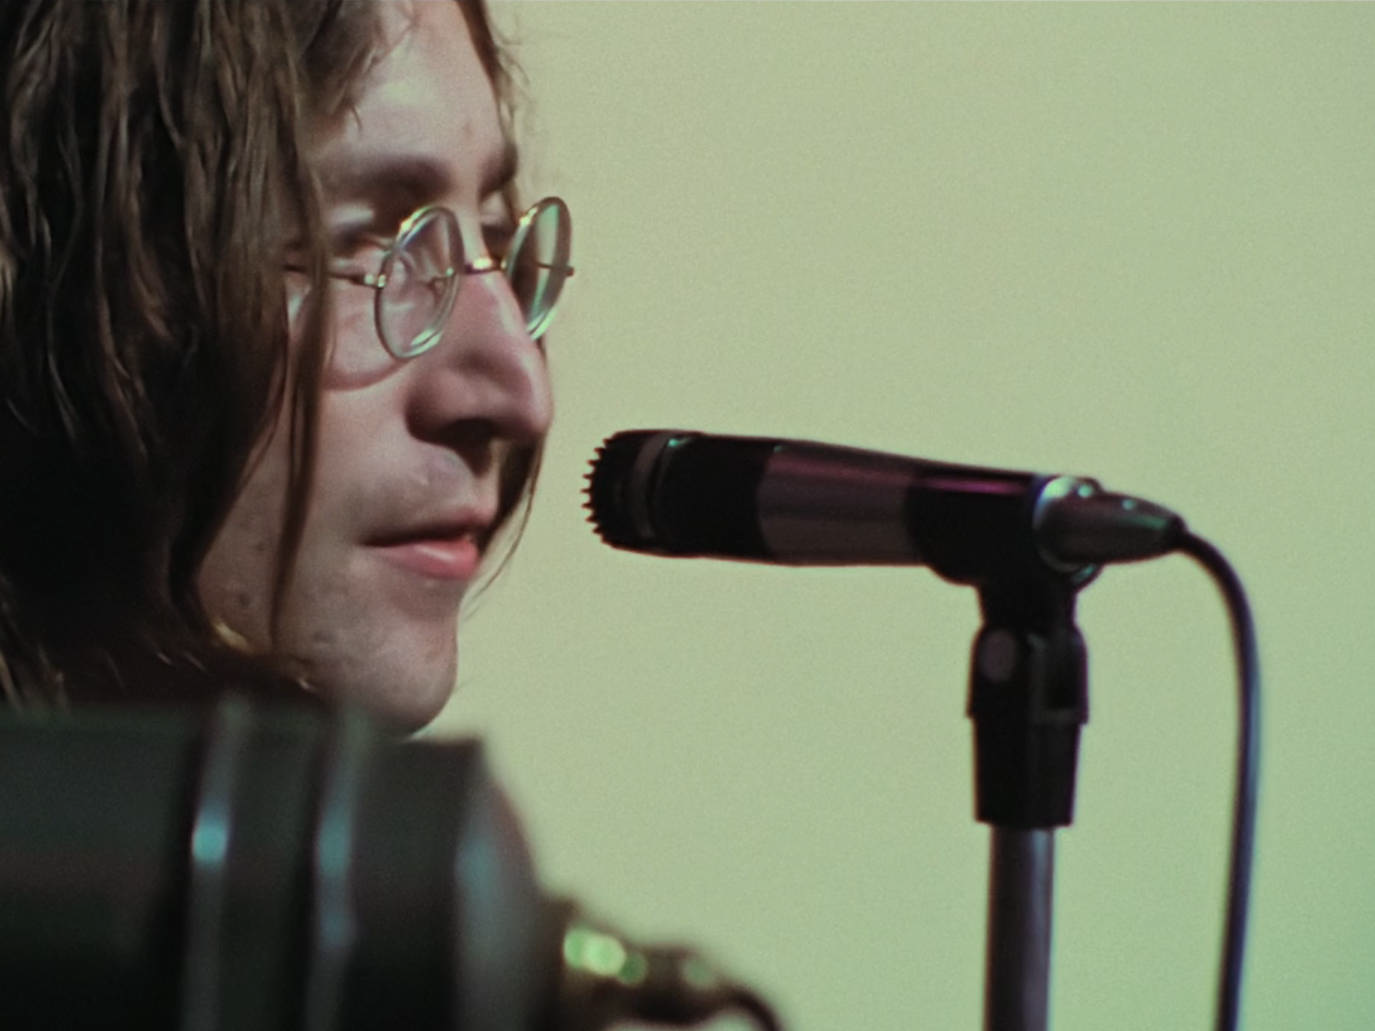
\includegraphics[width=\linewidth]{dflt/lennon_Q50_dec_dflt.png}
        \caption{Default Q=50.}
        
    \end{subfigure}
    \hfill
    \begin{subfigure}{0.30\textwidth}
        \centering
        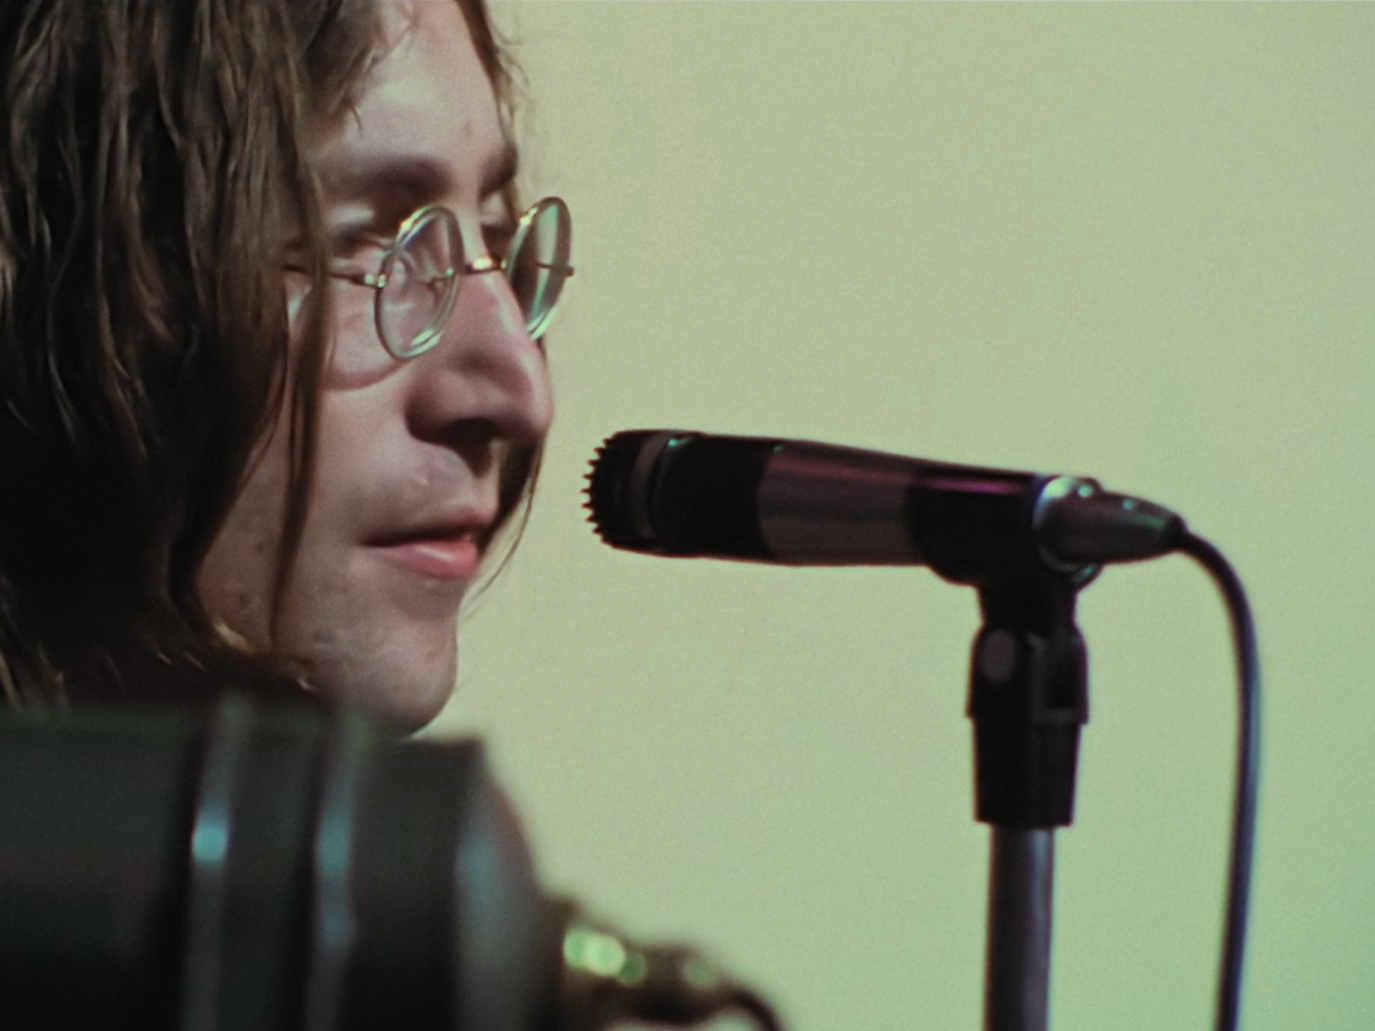
\includegraphics[width=\linewidth]{dflt/lennon_Q100_dec_dflt.png}
        \caption{Default Q=100.}
        
    \end{subfigure}
    \hfill
    \begin{subfigure}{0.30\textwidth}
        \centering
        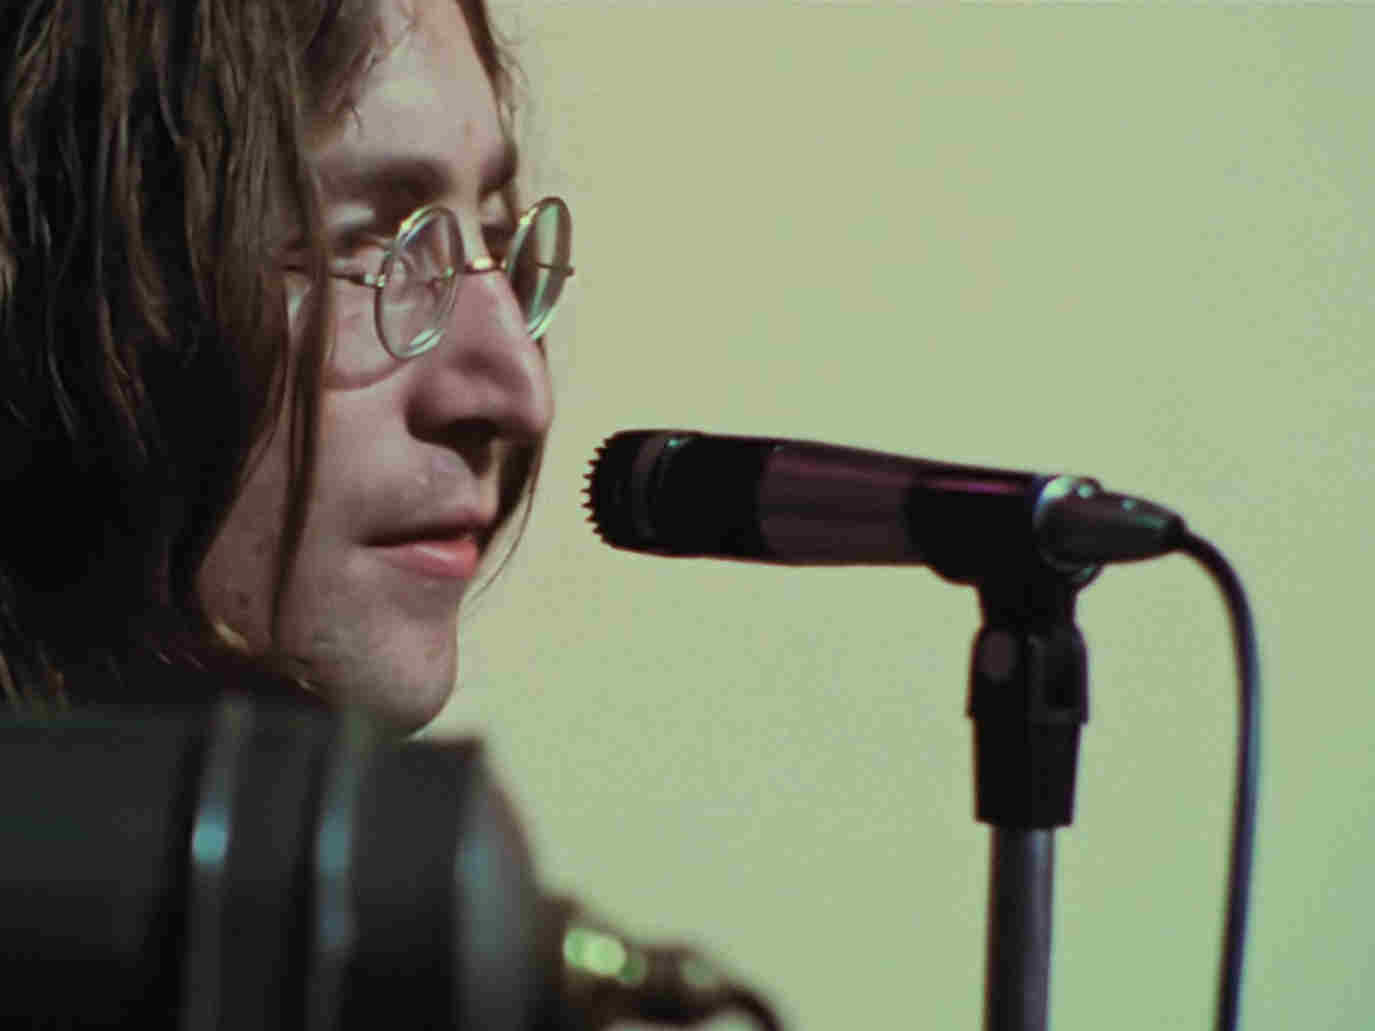
\includegraphics[width=\linewidth]{dflt/lennon_Q250_dec_dflt.png}
        \caption{Default Q=250.}
        
    \end{subfigure}
    
    \vspace{0.5cm}
    
    \begin{subfigure}{0.30\textwidth}
        \centering
        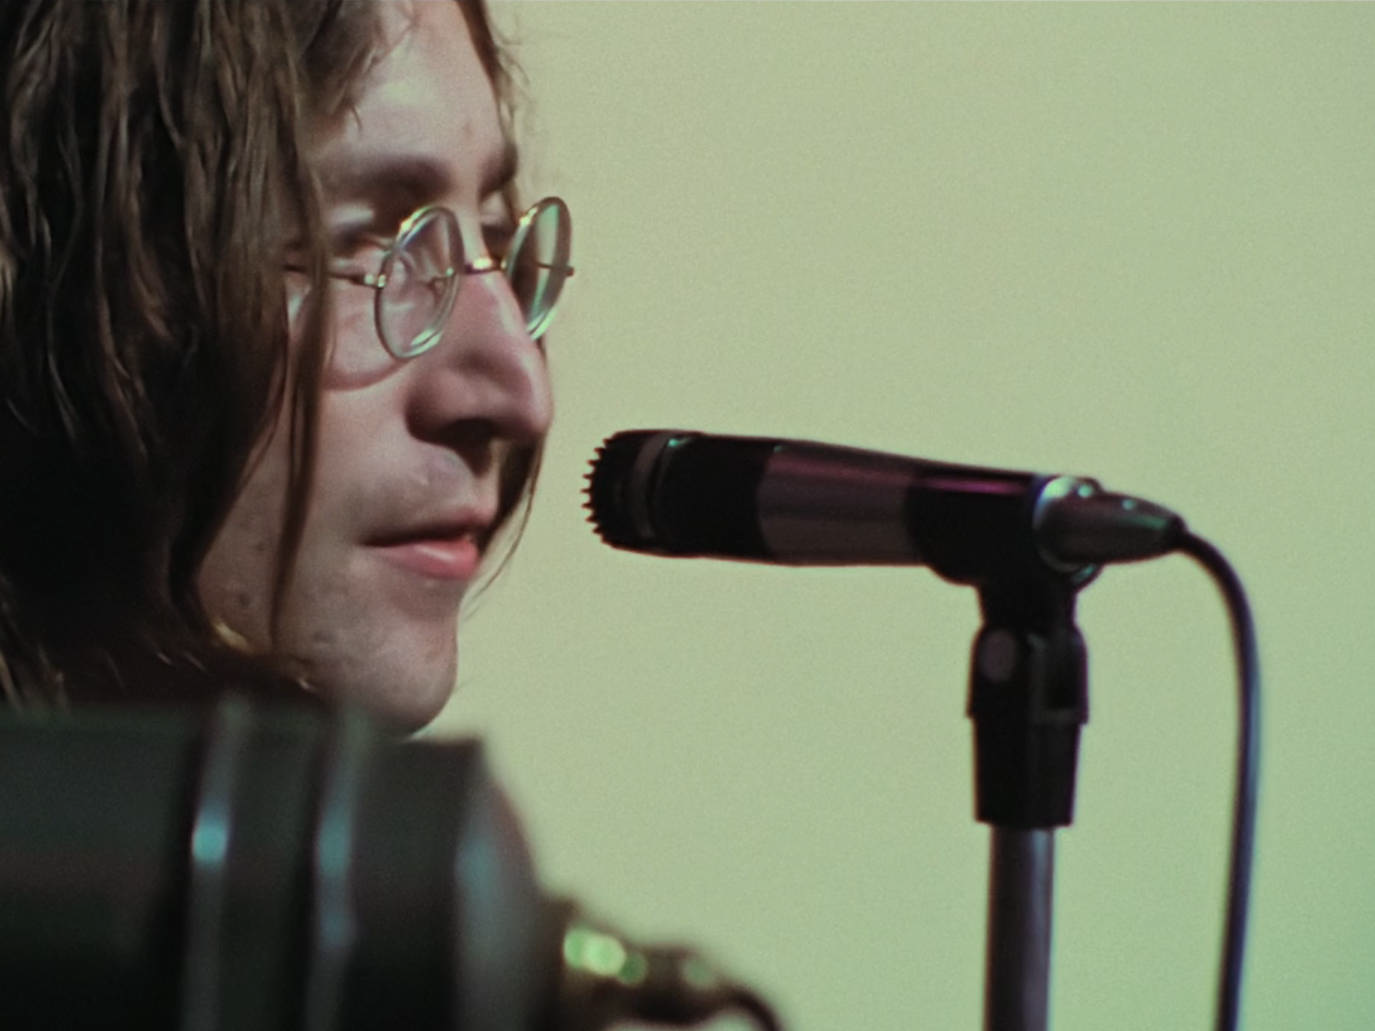
\includegraphics[width=\linewidth]{custom/lennon_Q50_dec_custom.png}
        \caption{Custom Q=50.}
        
    \end{subfigure}
    \hfill
    \begin{subfigure}{0.30\textwidth}
        \centering
        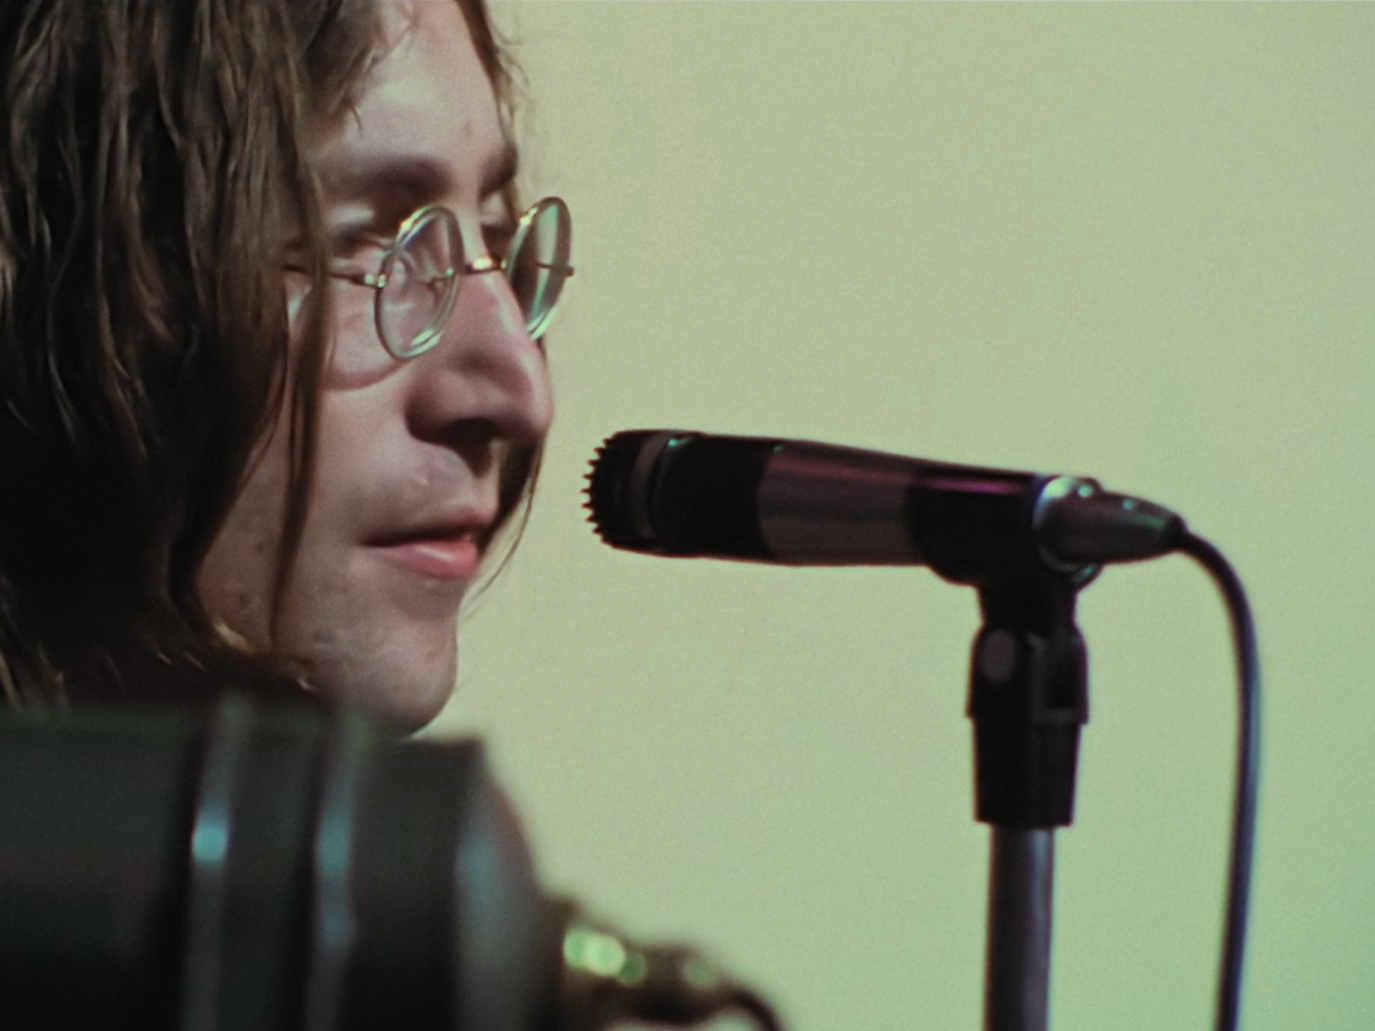
\includegraphics[width=\linewidth]{custom/lennon_Q100_dec_custom.png}
        \caption{Custom Q=100.}
        
    \end{subfigure}
    \hfill
    \begin{subfigure}{0.30\textwidth}
        \centering
        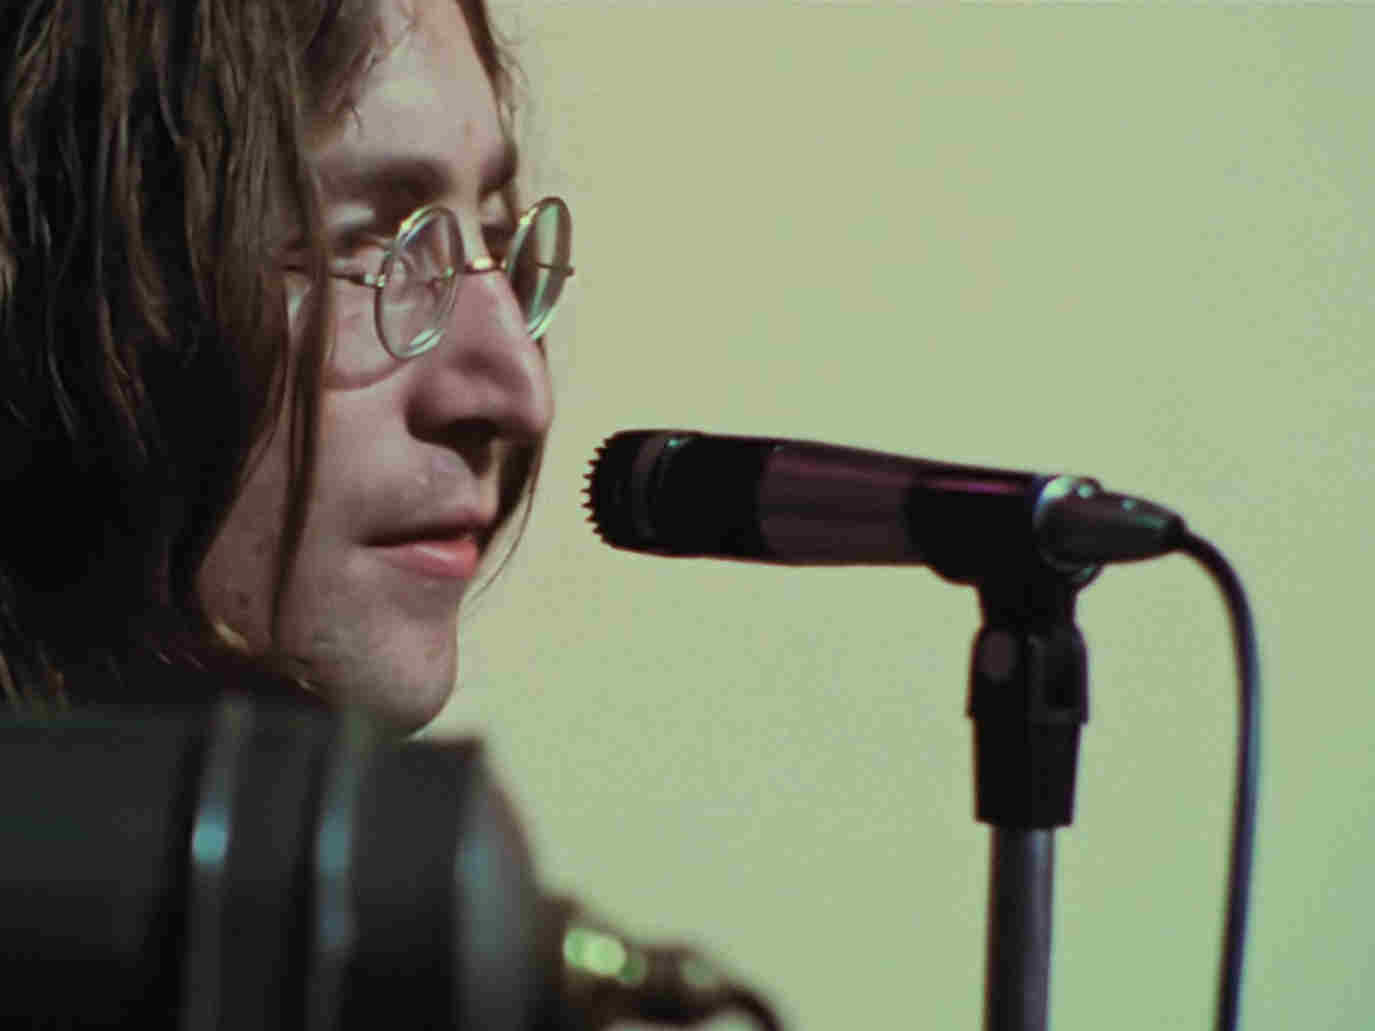
\includegraphics[width=\linewidth]{custom/lennon_Q250_dec_custom.png}
        \caption{Custom Q=250.}
        
    \end{subfigure}
    
    \caption[Resultados experimentales - lennon]{Resultados experimentales de la compresión de la imagen \textit{lennon.bmp}.}
    
\end{figure}

En esta imagen no aprecio diferencias muy notables entre los resultados con factor 50 y con factor 100. Los elementos principales de la imagen se siguen apreciando prácticamente igual, quizás debido a que la imagen original no tenía una gran cantidad de enfoque y una textura granulosa característica de las imágenes analógicas más antiguas (cuando más se notan las diferencias es cuando la imagen original tiene un enfoque muy nítido y texturas muy regulares, porque es de lo primero que se va perdiendo al comprimir la imagen). El fondo de la imagen empieza a unificarse en bloques del mismo color, pero al ser muy regular en la imagen original apenas sí se aprecia. Con factor 250 la imagen empeora notablemente. Adquiere una textura pixelada , aparecen manchas en la cara y el fondo se ve como grandes manchas de píxeles con una transición abrupta entre regiones. Elementos como el micrófono han perdido casi todos sus detalles, adquiriendo una textura plana.\\

Por estas razones escogeré el factor 100.




\subsubsection{graph}
Primero se muestra la imagen original para tener una referencia:
\begin{figure}[H]
    \centering
    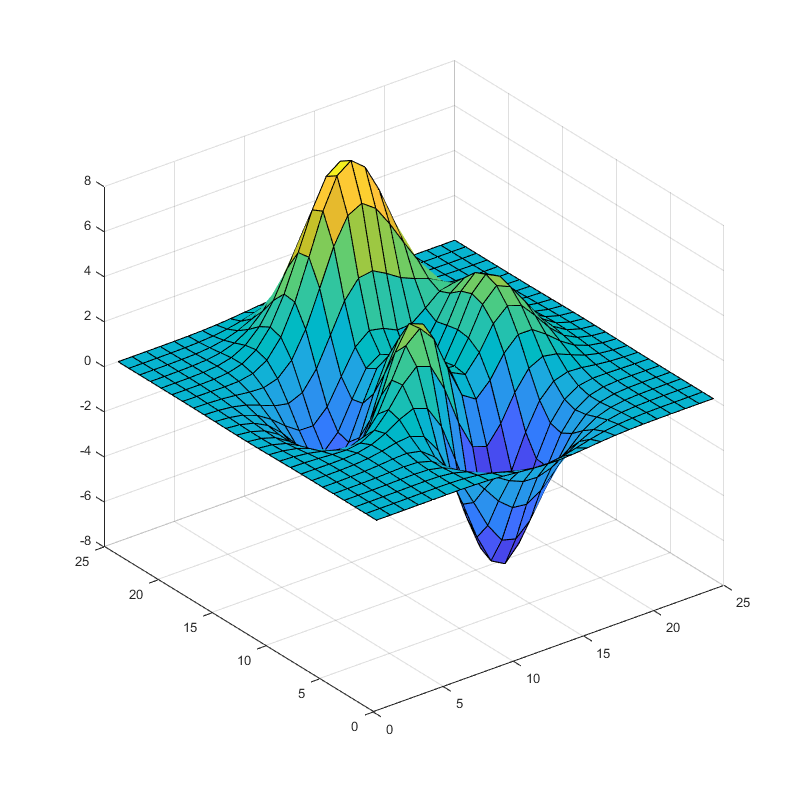
\includegraphics[width=0.30\textwidth]{images/graph.png}
    \caption[Referencia - graph]{Imagen original de referencia.}
    
\end{figure}
    \vspace{0.5cm}
    
Imágenes resultantes:
\begin{figure}   [H]
    \begin{subfigure}{0.30\textwidth}
        \centering
        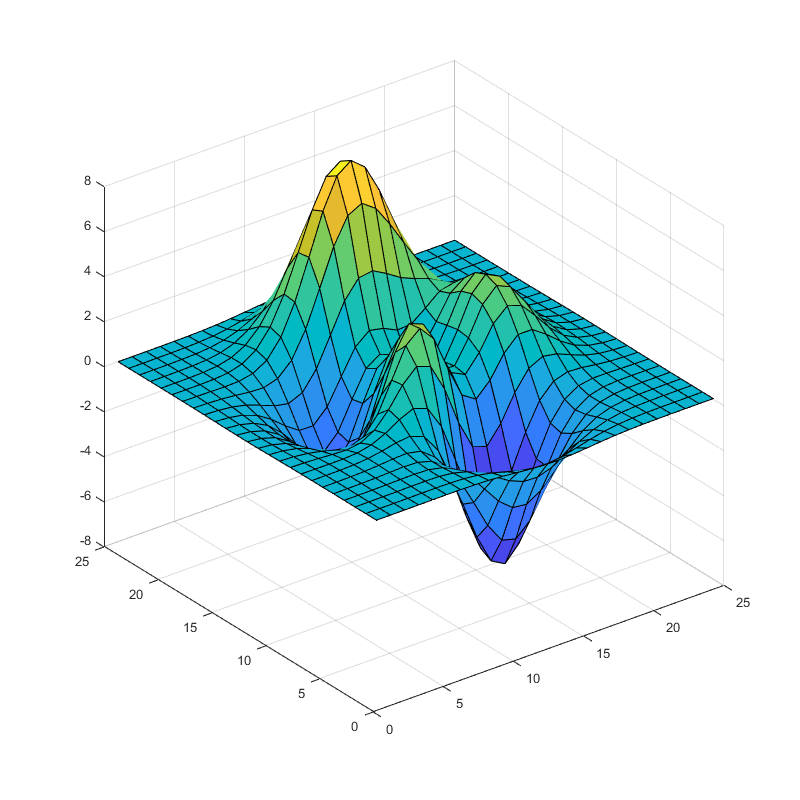
\includegraphics[width=\linewidth]{dflt/graph_Q50_dec_dflt.png}
        \caption{Default Q=50.}
        
    \end{subfigure}
    \hfill
    \begin{subfigure}{0.30\textwidth}
        \centering
        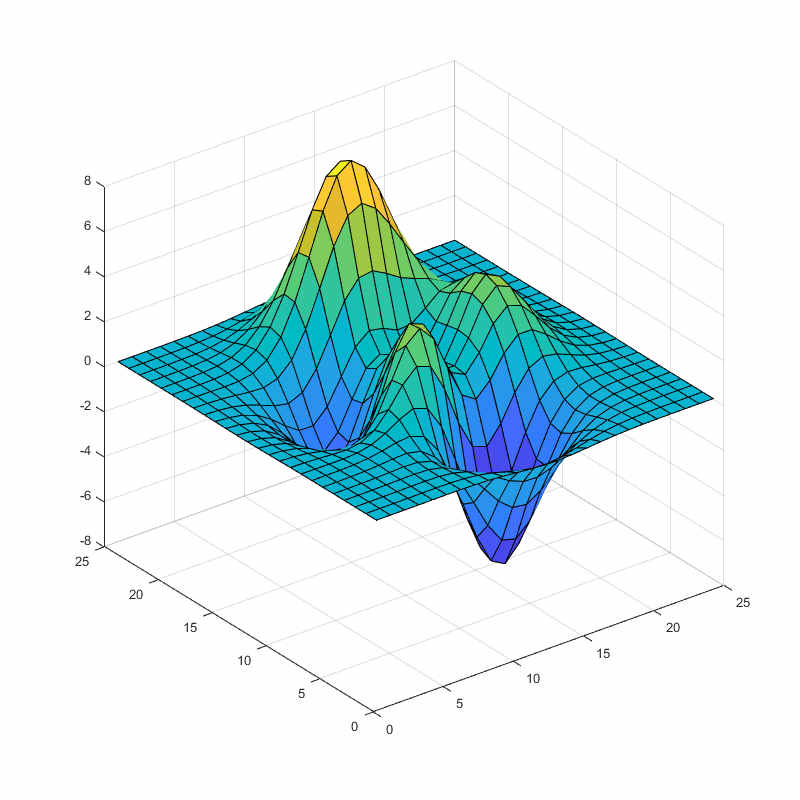
\includegraphics[width=\linewidth]{dflt/graph_Q100_dec_dflt.png}
        \caption{Default Q=100.}
        
    \end{subfigure}
    \hfill
    \begin{subfigure}{0.30\textwidth}
        \centering
        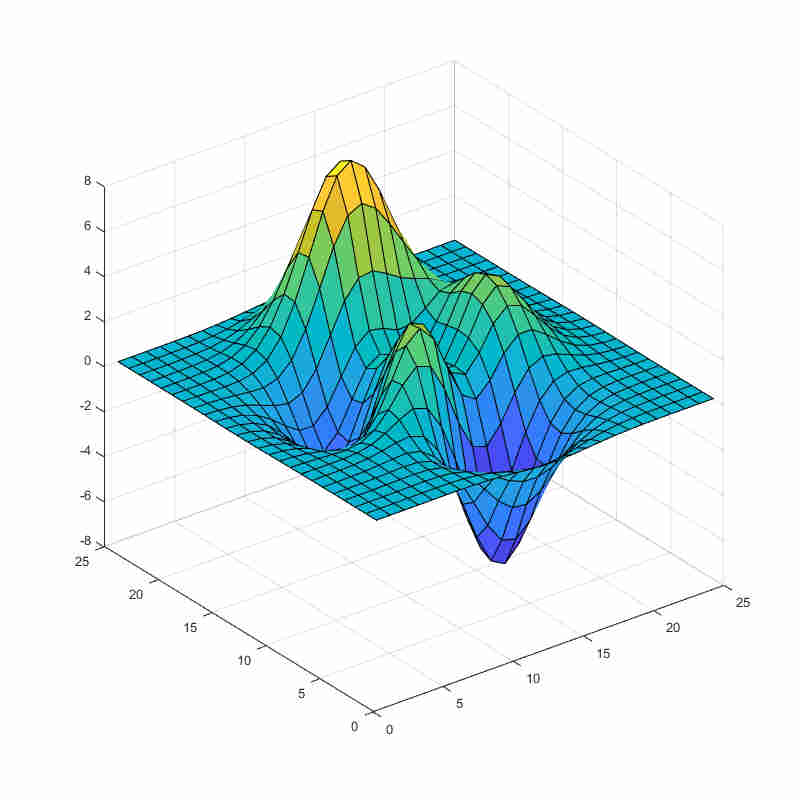
\includegraphics[width=\linewidth]{dflt/graph_Q250_dec_dflt.png}
        \caption{Default Q=250.}
        
    \end{subfigure}
    
    \vspace{0.5cm}
    
    \begin{subfigure}{0.30\textwidth}
        \centering
        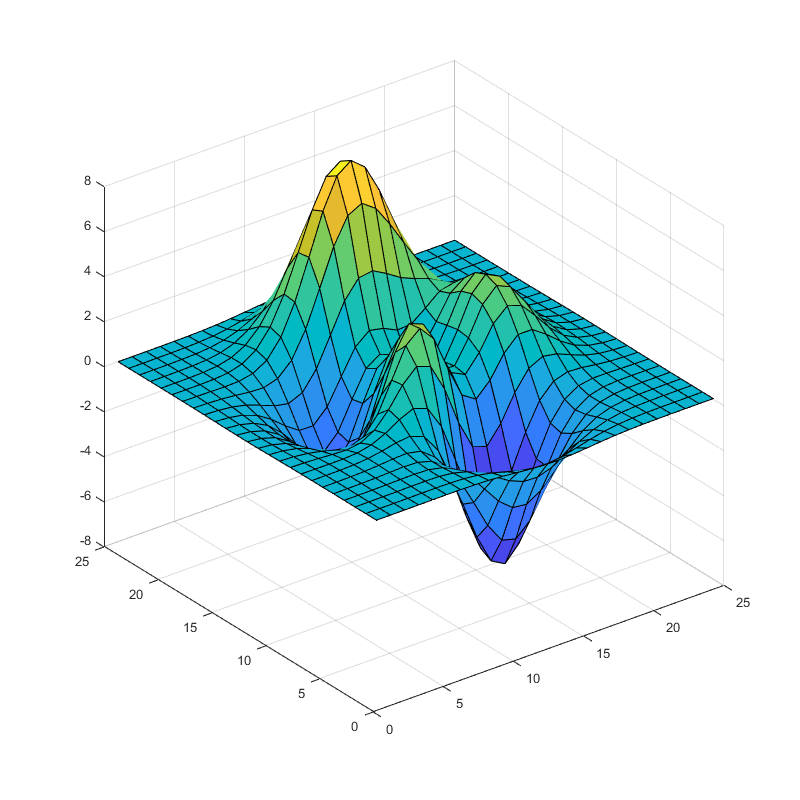
\includegraphics[width=\linewidth]{custom/graph_Q50_dec_custom.png}
        \caption{Custom Q=50.}
        
    \end{subfigure}
    \hfill
    \begin{subfigure}{0.30\textwidth}
        \centering
        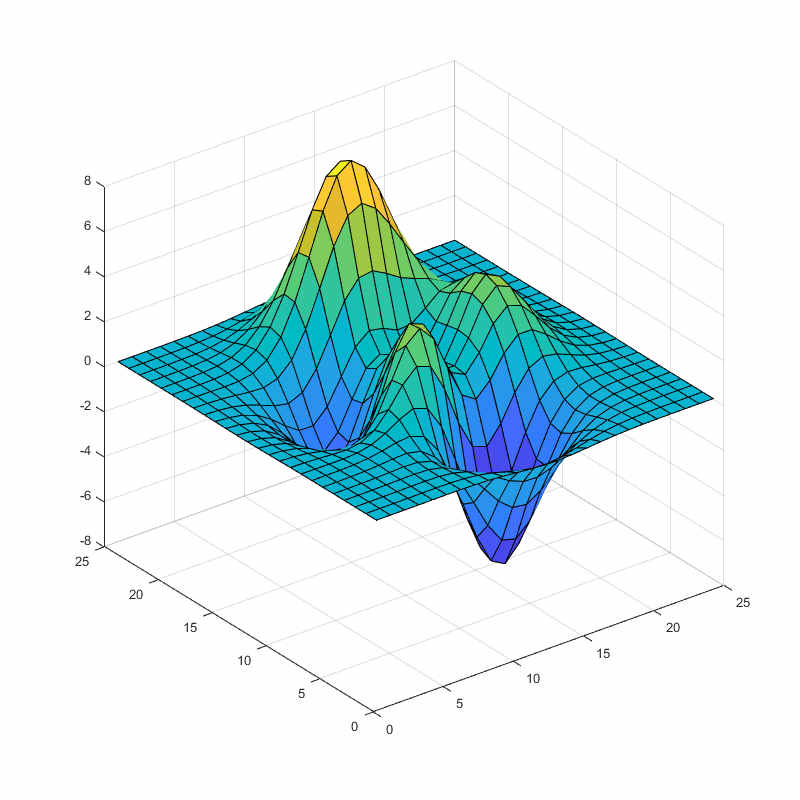
\includegraphics[width=\linewidth]{custom/graph_Q100_dec_custom.png}
        \caption{Custom Q=100.}
        
    \end{subfigure}
    \hfill
    \begin{subfigure}{0.30\textwidth}
        \centering
        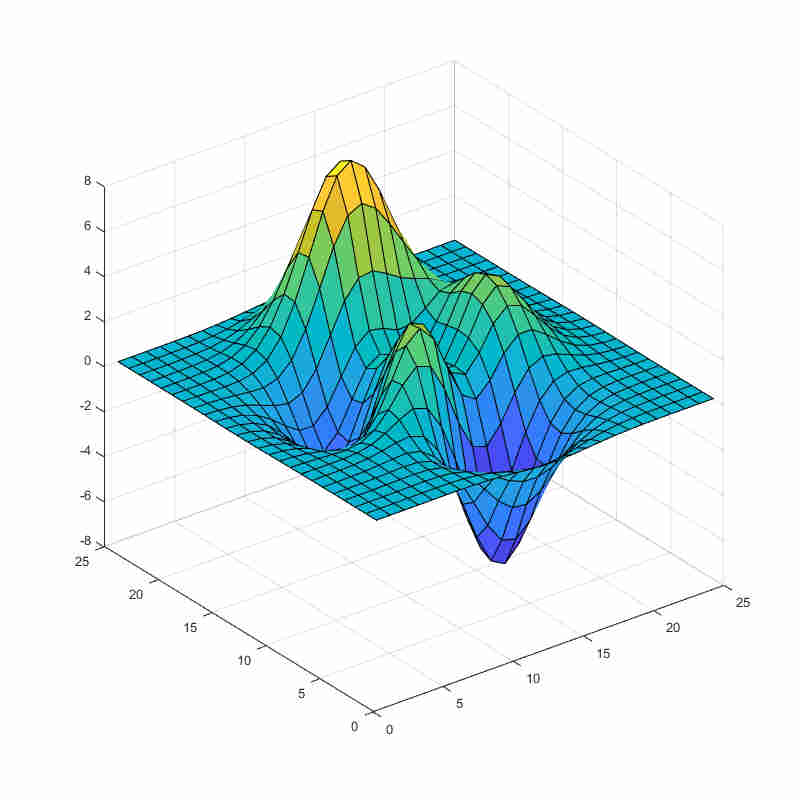
\includegraphics[width=\linewidth]{custom/graph_Q250_dec_custom.png}
        \caption{Custom Q=250.}
        
    \end{subfigure}
    
    \caption[Resultados experimentales - graph]{Resultados experimentales de la compresión de la imagen \textit{graph.bmp}.}
    
\end{figure}

Con factor 50 la diferencia más notable es que en los bordes de las casillas de la cuadrícula (que en la imagen original eran de un color uniforme) empiezan a aparecer pequeñas manchas de píxeles, intuyo que debido al cambio brusco de color respecto al negro de la línea de la cuadrícula. Con factor 100 este efecto es un poco más destacable, sobre todo en las casillas pequeñas, pero en general mantiene muy bien tanto los colores como las formas. Los números empiezan a emborronarse un poco y en general la imagen se ve menos nítida, pero nada demasiado destacable. En términos de visibilidad, se siguen apreciando perfectamente los ejes, las formas de la gráfica y sus colores. Con factor 250 el principal problema que encontramos es que empiezan a deformarse los contornos de la cuadrícula, porque en muchas casillas (sobre todo las más grandes) hay una región grande de un color uniforme que en algunos casos incluye el espacio donde debería estar la línea de la cuadrícula (visualmente parecen ``manchas gordas'' pegadas encima de las casillas, sin respetar las líneas de cuadrícula). Los ejes empiezan a difuminarse (el eje vertical se ve doble en algunos puntos) y algunos números no se leen bien. No considero que este resultado sea adecuado.\\

Para esta imagen voy a elegir el factor 100.\\


\subsubsection{lena}
Primero se muestra la imagen original para tener una referencia:
\begin{figure}[H]
    \centering
    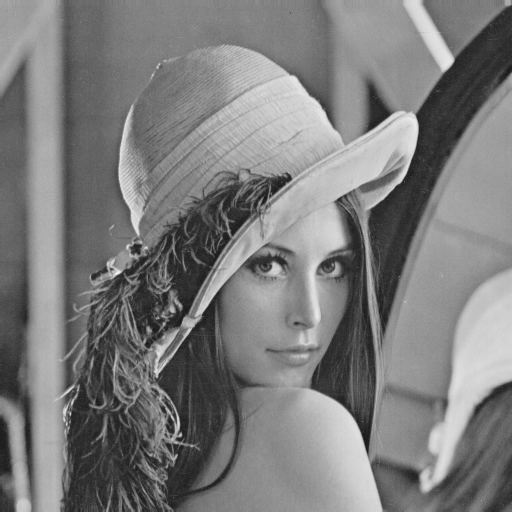
\includegraphics[width=0.30\textwidth]{images/lena.png}
    \caption[Referencia - lena]{Imagen original de referencia.}
    
\end{figure}
    
    \vspace{0.5cm}
    
Imágenes resultantes:
\begin{figure}   [H]
    \begin{subfigure}{0.30\textwidth}
        \centering
        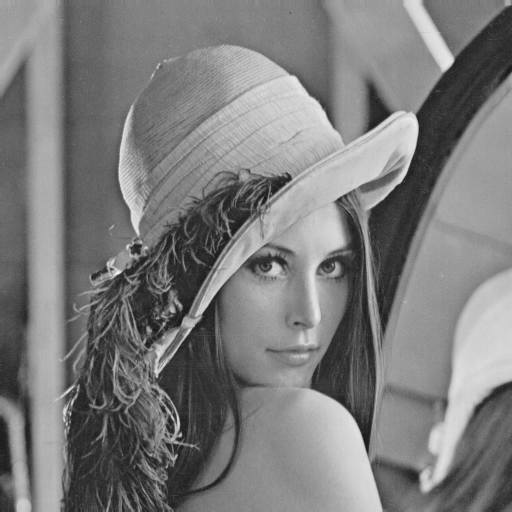
\includegraphics[width=\linewidth]{dflt/lena_Q50_dec_dflt.png}
        \caption{Default Q=50.}
        
    \end{subfigure}
    \hfill
    \begin{subfigure}{0.30\textwidth}
        \centering
        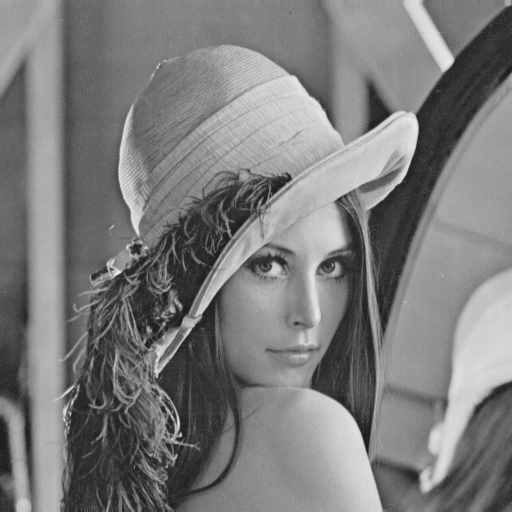
\includegraphics[width=\linewidth]{dflt/lena_Q100_dec_dflt.png}
        \caption{Default Q=100.}
        
    \end{subfigure}
    \hfill
    \begin{subfigure}{0.30\textwidth}
        \centering
        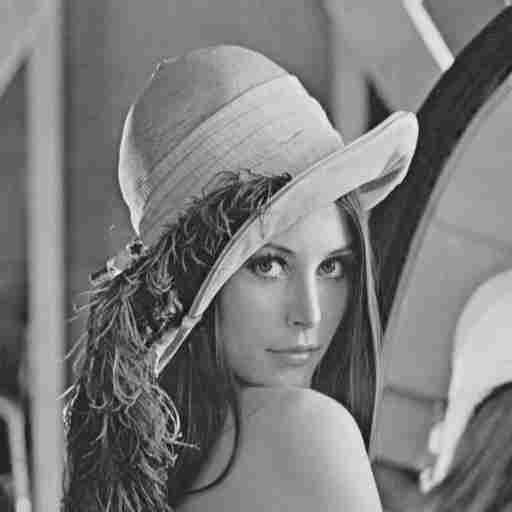
\includegraphics[width=\linewidth]{dflt/lena_Q250_dec_dflt.png}
        \caption{Default Q=250.}
        
    \end{subfigure}
    
    \vspace{0.5cm}
    
    \begin{subfigure}{0.30\textwidth}
        \centering
        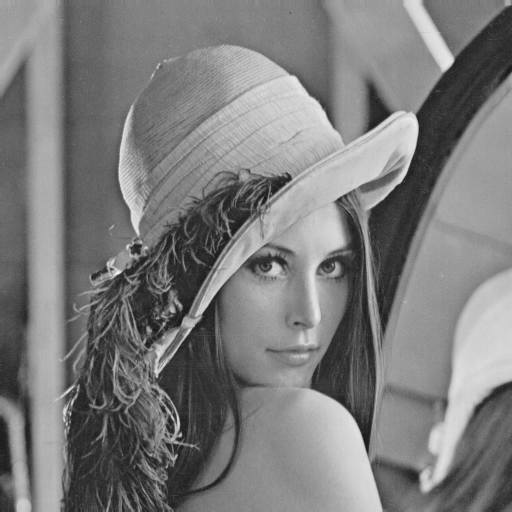
\includegraphics[width=\linewidth]{custom/lena_Q50_dec_custom.png}
        \caption{Custom Q=50.}
        
    \end{subfigure}
    \hfill
    \begin{subfigure}{0.30\textwidth}
        \centering
        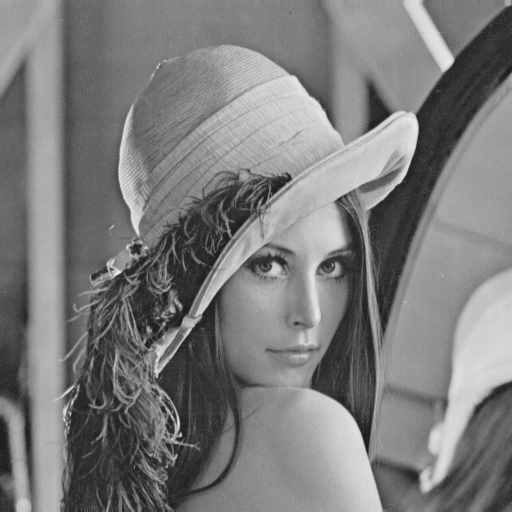
\includegraphics[width=\linewidth]{custom/lena_Q100_dec_custom.png}
        \caption{Custom Q=100.}
        
    \end{subfigure}
    \hfill
    \begin{subfigure}{0.30\textwidth}
        \centering
        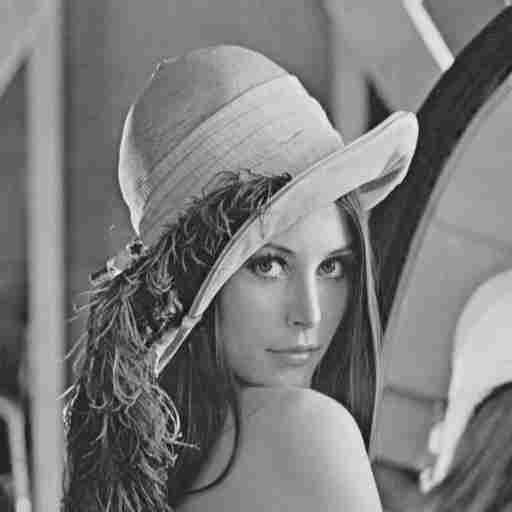
\includegraphics[width=\linewidth]{custom/lena_Q250_dec_custom.png}
        \caption{Custom Q=250.}
        
    \end{subfigure}
    
    \caption[Resultados experimentales - lena]{Resultados experimentales de la compresión de la imagen \textit{lena.bmp}.}
    
\end{figure}

En esta imagen los resultados son bastante buenos, y la diferencia entre el factor 50 y el factor 100 es mínima, y apenas se pierden detalles respecto a la imagen original. Con factor 250 la imagen adquiere la textura pixelada que ya hemos comentado en las imágenes anteriores y en el fondo aparecen manchas uniformes muy apreciables.\\ 

En este caso elegiré también el factor 100.

\subsubsection{mandrill}
Primero se muestra la imagen original para tener una referencia:
\begin{figure}[H]
    \centering
    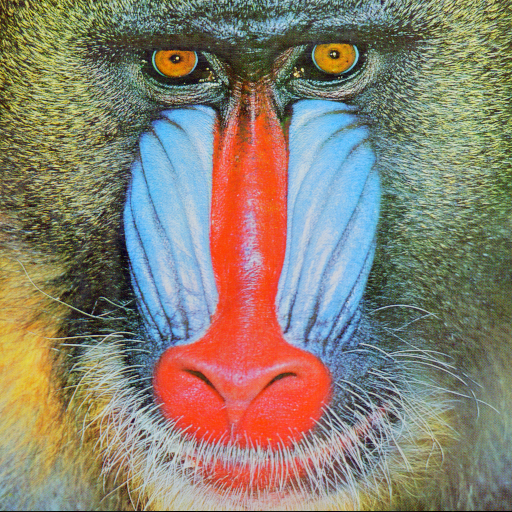
\includegraphics[width=0.30\textwidth]{images/mandrill.png}
    \caption[Referencia - mandrill]{Imagen original de referencia.}
    
\end{figure}
    
    \vspace{0.5cm}

Imágenes resultantes:
\begin{figure}   [H]
    \begin{subfigure}{0.30\textwidth}
        \centering
        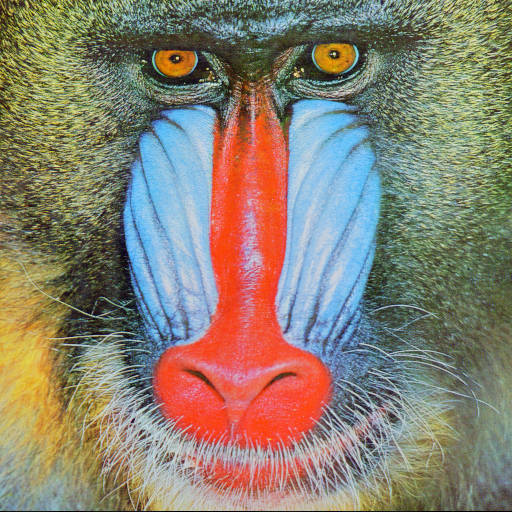
\includegraphics[width=\linewidth]{dflt/mandrill_Q50_dec_dflt.png}
        \caption{Default Q=50.}
        
    \end{subfigure}
    \hfill
    \begin{subfigure}{0.30\textwidth}
        \centering
        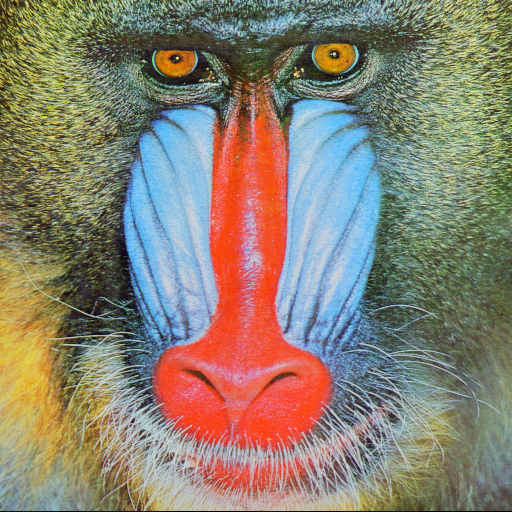
\includegraphics[width=\linewidth]{dflt/mandrill_Q100_dec_dflt.png}
        \caption{Default Q=100.}
        
    \end{subfigure}
    \hfill
    \begin{subfigure}{0.30\textwidth}
        \centering
        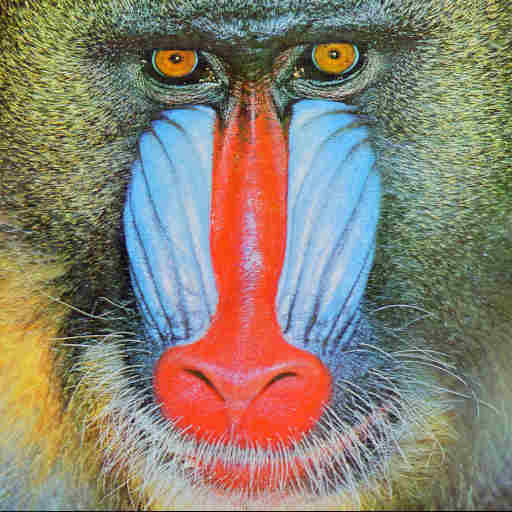
\includegraphics[width=\linewidth]{dflt/mandrill_Q250_dec_dflt.png}
        \caption{Default Q=250.}
        
    \end{subfigure}
    
    \vspace{0.5cm}
    
    \begin{subfigure}{0.30\textwidth}
        \centering
        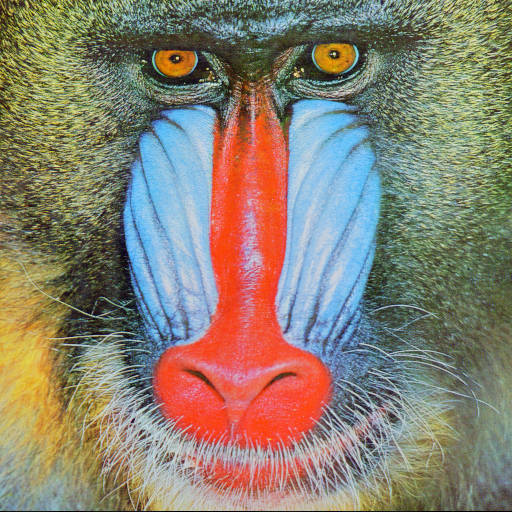
\includegraphics[width=\linewidth]{custom/mandrill_Q50_dec_custom.png}
        \caption{Custom Q=50.}
        
    \end{subfigure}
    \hfill
    \begin{subfigure}{0.30\textwidth}
        \centering
        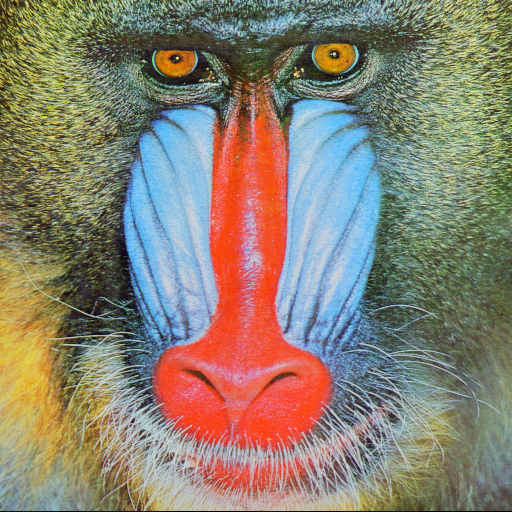
\includegraphics[width=\linewidth]{custom/mandrill_Q100_dec_custom.png}
        \caption{Custom Q=100.}
        
    \end{subfigure}
    \hfill
    \begin{subfigure}{0.30\textwidth}
        \centering
        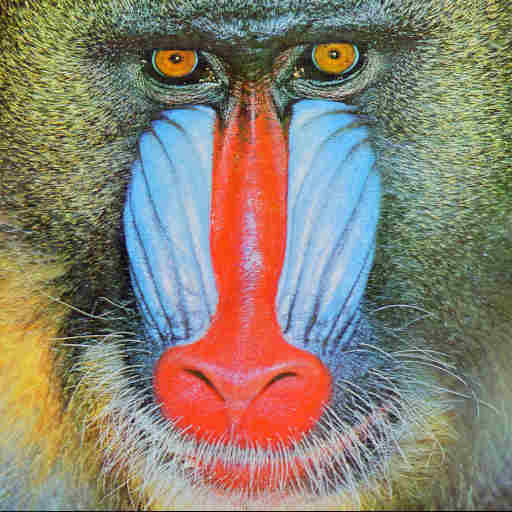
\includegraphics[width=\linewidth]{custom/mandrill_Q250_dec_custom.png}
        \caption{Custom Q=250.}
        
    \end{subfigure}
    
    \caption[Resultados experimentales - mandrill]{Resultados experimentales de la compresión de la imagen \textit{mandrill.bmp}.}
    
\end{figure}


\subsubsection{noise}
Primero se muestra la imagen original para tener una referencia:
\begin{figure}[H]
    \centering
    
\includegraphics[width=0.30\textwidth]{images/noise.png}
    \caption[Referencia - noise]{Imagen original de referencia.}
    
\end{figure}
    
    \vspace{0.5cm}

Imágenes resultantes:
\begin{figure}   [H]
    \begin{subfigure}{0.30\textwidth}
        \centering
        
\includegraphics[width=\linewidth]{dflt/noise_Q50_dec_dflt.png}
        \caption{Default Q=50.}
        
    \end{subfigure}
    \hfill
    \begin{subfigure}{0.30\textwidth}
        \centering
        
\includegraphics[width=\linewidth]{dflt/noise_Q100_dec_dflt.png}
        \caption{Default Q=100.}
        
    \end{subfigure}
    \hfill
    \begin{subfigure}{0.30\textwidth}
        \centering
        
\includegraphics[width=\linewidth]{dflt/noise_Q250_dec_dflt.png}
        \caption{Default Q=250.}
        
    \end{subfigure}
    
    \vspace{0.5cm}
    
    \begin{subfigure}{0.30\textwidth}
        \centering
        \includegraphics[width=\linewidth]{custom/noise_Q50_dec_custom.png}
        \caption{Custom Q=50.}
        
    \end{subfigure}
    \hfill
    \begin{subfigure}{0.30\textwidth}
        \centering
        \includegraphics[width=\linewidth]{custom/noise_Q100_dec_custom.png}
        \caption{Custom Q=100.}
        
    \end{subfigure}
    \hfill
    \begin{subfigure}{0.30\textwidth}
        \centering
        \includegraphics[width=\linewidth]{custom/noise_Q250_dec_custom.png}
        \caption{Custom Q=250.}
        
    \end{subfigure}
    
    \caption[Resultados experimentales - noise]{Resultados experimentales de la compresión de la imagen \textit{noise.bmp}.}
    
\end{figure}

Esta imagen es un poco difícil de analizar debido a que no hay formas ni contornos reconocibles. No aprecio ninguna diferencia entre el factor 50 y el factor 100. En el factor 250 ya noto como la imagen se agrupa en bloques de píxeles bien diferenciados. Será interesante ver las diferencias cuantitativas entre los dos primeros factores de calidad.\\

Elijo el factor 100.


\subsubsection{pattern}
Primero se muestra la imagen original para tener una referencia:
\begin{figure}[H]
    \centering
    \includegraphics[width=0.30\textwidth]{images/pattern.png}
    \caption[Referencia - pattern]{Imagen original de referencia.}
    
\end{figure}
    \vspace{0.5cm}

Imágenes resultantes:
\begin{figure}[H]

    \begin{subfigure}{0.30\textwidth}
        \centering
        \includegraphics[width=\linewidth]{dflt/pattern_Q50_dec_dflt.png}
        \caption{Default Q=50.}
        
    \end{subfigure}
    \hfill
    \begin{subfigure}{0.30\textwidth}
        \centering
        \includegraphics[width=\linewidth]{dflt/pattern_Q100_dec_dflt.png}
        \caption{Default Q=100.}
        
    \end{subfigure}
    \hfill
    \begin{subfigure}{0.30\textwidth}
        \centering
        \includegraphics[width=\linewidth]{dflt/pattern_Q250_dec_dflt.png}
        \caption{Default Q=250.}
        
    \end{subfigure}
    
    \vspace{0.5cm}
    
    \begin{subfigure}{0.30\textwidth}
        \centering
        \includegraphics[width=\linewidth]{custom/pattern_Q50_dec_custom.png}
        \caption{Custom Q=50.}
        
    \end{subfigure}
    \hfill
    \begin{subfigure}{0.30\textwidth}
        \centering
        \includegraphics[width=\linewidth]{custom/pattern_Q100_dec_custom.png}
        \caption{Custom Q=100.}
        
    \end{subfigure}
    \hfill
    \begin{subfigure}{0.30\textwidth}
        \centering
        \includegraphics[width=\linewidth]{custom/pattern_Q250_dec_custom.png}
        \caption{Custom Q=250.}
        
    \end{subfigure}
    
    \caption[Resultados experimentales - pattern]{Resultados experimentales de la compresión de la imagen \textit{pattern.bmp}.}
    
\end{figure}

Con el factor 50 vemos que el patrón de la imagen se mantiene casi inalterado (salvo algunos píxeles que adquieren una tonalidad de gris casi inapreciable). Con factor 100 aparecen píxeles gris oscuro casi negro de forma regular en algunas zonas del patrón. Con factor 250 aparte de lo anterior muchos píxeles blancos adquieren distintas tonalidades de gris . Mientras que se aprecian los elementos más importantes del patrón original, en general se diferencia bastante.\\

Es interesante destacar que, debido a la presencia de un patrón que se repite periódicamente, los cambios respecto a la imagen original se producen de forma uniforme dentro de cada elemento constitutivo base del patrón. Es decir, los cambios son ``locales'' a nivel de cada elemento del patrón.\\

Aunque pueda resultar anti intuitivo en este caso escogeré el factor 50. Considero que lo importante de esta imagen es el patrón concreto de píxeles que la forma. Con el factor 100 ya se introducen cambios significativos con los que podríamos decir que es un patrón diferente, así que no lo considero adecuado. \\

\subsubsection{color\_bars}
Primero se muestra la imagen original para tener una referencia:
\begin{figure}[H]
    \centering
    \includegraphics[width=0.30\textwidth]{images/color_bars.png}
    \caption[Referencia - color\_bars]{Imagen original de referencia.}
    
\end{figure}

\vspace{0.5cm}

Imágenes resultantes:
\begin{figure}   [H]
    \begin{subfigure}{0.30\textwidth}
        \centering
        \includegraphics[width=\linewidth]{dflt/color_bars_Q100_dec_dflt.png}
        \caption{Default Q=100.}
        
    \end{subfigure}
    \hfill
    \begin{subfigure}{0.30\textwidth}
        \centering
        \includegraphics[width=\linewidth]{dflt/color_bars_Q500_dec_dflt.png}
        \caption{Default Q=500.}
        
    \end{subfigure}
    \hfill
    \begin{subfigure}{0.30\textwidth}
        \centering
        \includegraphics[width=\linewidth]{dflt/color_bars_Q1000_dec_dflt.png}
        \caption{Default Q=1000.}
        
    \end{subfigure}
    
    \vspace{0.5cm}
    
    \begin{subfigure}{0.30\textwidth}
        \centering
        \includegraphics[width=\linewidth]{custom/color_bars_Q100_dec_custom.png}
        \caption{Custom Q=100.}
        
    \end{subfigure}
    \hfill
    \begin{subfigure}{0.30\textwidth}
        \centering
        \includegraphics[width=\linewidth]{custom/color_bars_Q500_dec_custom.png}
        \caption{Custom Q=500.}
        
    \end{subfigure}
    \hfill
    \begin{subfigure}{0.30\textwidth}
        \centering
        \includegraphics[width=\linewidth]{custom/color_bars_Q1000_dec_custom.png}
        \caption{Custom Q=1000.}
        
    \end{subfigure}
    
    \caption[Resultados experimentales - color\_bars]{Resultados experimentales de la compresión de la imagen \textit{color\_bars.bmp}.}
    
\end{figure}

Como hemos señalado en secciones anteriores, este caso es especial puesto que estamos en un caso muy favorable para estos compresores que estamos utilizando. Por esa razón analizaremos en este caso factores de calidad mucho más altos.\\

Con factor 100 las diferencias son inexistentes, pero es que sucede lo mismo con el factor 500. De hecho, al pasar al factor 1000 la única diferencia notable la encontramos en la tonalidad de la primera barra, la de color blanco, que adquiere un tono grisáceo. Es muy destacable que, pese a los cambios bruscos de color entre las distintas regiones, los contornos no se han visto nada modificados, ni en el factor de calidad más elevado. Esto concuerda con nuestra hipótesis previa basada en el funcionamiento del compresor DCT.\\

A falta de analizar los resultados cuantitativos, podemos decir que la calidad visual que se preserva es increíble. Por estas razones, escogeré el factor 500.\\

\subsubsection{explorer}
Primero se muestra la imagen original para tener una referencia:
\begin{figure}[H]
    \centering
    \includegraphics[width=0.30\textwidth]{images/explorer.png}
    \caption[Referencia - explorer]{Imagen original de referencia.}
    
\end{figure}
    
    \vspace{0.5cm}

Imágenes resultantes:
\begin{figure}[H]
    
    \begin{subfigure}{0.30\textwidth}
        \centering
        \includegraphics[width=\linewidth]{dflt/explorer_Q50_dec_dflt.png}
        \caption{Default Q=50.}
        
    \end{subfigure}
    \hfill
    \begin{subfigure}{0.30\textwidth}
        \centering
        \includegraphics[width=\linewidth]{dflt/explorer_Q100_dec_dflt.png}
        \caption{Default Q=100.}
        
    \end{subfigure}
    \hfill
    \begin{subfigure}{0.30\textwidth}
        \centering
        \includegraphics[width=\linewidth]{dflt/explorer_Q250_dec_dflt.png}
        \caption{Default Q=250.}
        
    \end{subfigure}
    
    \vspace{0.5cm}
    
    \begin{subfigure}{0.30\textwidth}
        \centering
        \includegraphics[width=\linewidth]{custom/explorer_Q50_dec_custom.png}
        \caption{Custom Q=50.}
        
    \end{subfigure}
    \hfill
    \begin{subfigure}{0.30\textwidth}
        \centering
        \includegraphics[width=\linewidth]{custom/explorer_Q100_dec_custom.png}
        \caption{Custom Q=100.}
        
    \end{subfigure}
    \hfill
    \begin{subfigure}{0.30\textwidth}
        \centering
        \includegraphics[width=\linewidth]{custom/explorer_Q250_dec_custom.png}
        \caption{Custom Q=250.}
        
    \end{subfigure}
    
    \caption[Resultados experimentales - explorer]{Resultados experimentales de la compresión de la imagen \textit{explorer.bmp}.}
    
\end{figure}

Con factor 50 vemos ya cómo el texto se emborrona y aparece una especie de ``halo de píxeles'' alrededor de las letras. El fondo se preserva plano, pero en los elementos como el texto o los iconos se aprecia bastante este efecto que puede dificultar la lectura. Con factor 100 se acentúa este efecto y algunas líneas como la de la barra de direcciones se empiezan a ver dobles. Las palabras podrían ser difícilmente legibles para personas con algún problema de visión. Con factor 250 cuesta distinguir algunas palabras, y elementos gráficos como la chincheta de la barra de acceso rápido son totalmente indistinguibles.\\

Debido a que aquí lo importante es la legibilidad del texto, y vemos que empeora rápidamente, me quedaré con el factor 50.\\

\subsubsection{gradient}
Primero se muestra la imagen original para tener una referencia:
\begin{figure}[H]
    \centering
    \includegraphics[width=0.25\textwidth]{images/gradient.png}
    \caption[Referencia - gradient]{Imagen original de referencia.}
    
\end{figure}
    
    \vspace{0.5cm}

Imágenes resultantes:
\begin{figure}[H]
    
    \begin{subfigure}{0.25\textwidth}
        \centering
        \includegraphics[width=\linewidth]{dflt/gradient_Q50_dec_dflt.png}
        \caption{Default Q=50.}
        
    \end{subfigure}
    \hfill
    \begin{subfigure}{0.25\textwidth}
        \centering
        \includegraphics[width=\linewidth]{dflt/gradient_Q100_dec_dflt.png}
        \caption{Default Q=100.}
        
    \end{subfigure}
    \hfill
    \begin{subfigure}{0.25\textwidth}
        \centering
        \includegraphics[width=\linewidth]{dflt/gradient_Q250_dec_dflt.png}
        \caption{Default Q=250.}
        
    \end{subfigure}
    
    \vspace{0.5cm}
    
    \begin{subfigure}{0.25\textwidth}
        \centering
        \includegraphics[width=\linewidth]{custom/gradient_Q50_dec_custom.png}
        \caption{Custom Q=50.}
        
    \end{subfigure}
    \hfill
    \begin{subfigure}{0.25\textwidth}
        \centering
        \includegraphics[width=\linewidth]{custom/gradient_Q100_dec_custom.png}
        \caption{Custom Q=100.}
        
    \end{subfigure}
    \hfill
    \begin{subfigure}{0.25\textwidth}
        \centering
        \includegraphics[width=\linewidth]{custom/gradient_Q250_dec_custom.png}
        \caption{Custom Q=250.}
        
    \end{subfigure}
    
    \caption[Resultados experimentales - gradient]{Resultados experimentales de la compresión de la imagen \textit{gradient.bmp}.}
    
\end{figure}

En este caso vemos cómo los resultados coinciden en gran medida con la hipótesis planteada. De la transición gradual y suave de la imagen original se pasa a transiciones de color cada vez más abruptas en regiones escalonadas del mismo color. Es decir, colores parecidos se agrupan en una sola región de un colo único, y el tamaño de esta región crece conforme lo hace Q.\\

Con factor 50 la transición sigue siendo suave y casi imperceptible. Con factor 100 se empieza a ver una textura un poco pixelada y una transición un poco menos suave, pero el efecto se nota poco. Con factor 250 las transiciones son muy abruptas y el resultado no es adecuado visualmente.\\

Elegiré en este caso el factor 100.

\subsubsection{color\_shapes}
Primero se muestra la imagen original para tener una referencia:
\begin{figure}[H]
    \centering
    \includegraphics[width=0.30\textwidth]{images/cshapes.png}
    \caption[Referencia - color\_shapes]{Imagen original de referencia.}
    
\end{figure}
    
    \vspace{0.5cm}

Imágenes resultantes:
\begin{figure}[H]
    
    \begin{subfigure}{0.30\textwidth}
        \centering
        \includegraphics[width=\linewidth]{dflt/cshapes_Q50_dec_dflt.png}
        \caption{Default Q=50.}
        
    \end{subfigure}
    \hfill
    \begin{subfigure}{0.30\textwidth}
        \centering
        \includegraphics[width=\linewidth]{dflt/cshapes_Q100_dec_dflt.png}
        \caption{Default Q=100.}
        
    \end{subfigure}
    \hfill
    \begin{subfigure}{0.30\textwidth}
        \centering
        \includegraphics[width=\linewidth]{dflt/cshapes_Q250_dec_dflt.png}
        \caption{Default Q=250.}
        
    \end{subfigure}
    
    \vspace{0.5cm}
    
    \begin{subfigure}{0.30\textwidth}
        \centering
        \includegraphics[width=\linewidth]{custom/cshapes_Q50_dec_custom.png}
        \caption{Custom Q=50.}
        
    \end{subfigure}
    \hfill
    \begin{subfigure}{0.30\textwidth}
        \centering
        \includegraphics[width=\linewidth]{custom/cshapes_Q100_dec_custom.png}
        \caption{Custom Q=100.}
        
    \end{subfigure}
    \hfill
    \begin{subfigure}{0.30\textwidth}
        \centering
        \includegraphics[width=\linewidth]{custom/cshapes_Q250_dec_custom.png}
        \caption{Custom Q=250.}
        
    \end{subfigure}
    
    \caption[Resultados experimentales - color\_shapes]{Resultados experimentales de la compresión de la imagen \textit{cshapes.bmp}.}
    
\end{figure}


\subsubsection{x-ray}
Primero se muestra la imagen original para tener una referencia:
\begin{figure}[H]
    \centering
    \includegraphics[width=0.30\textwidth]{images/xray.png}
    \caption[Referencia - x-ray]{Imagen original de referencia.}
    
\end{figure}
    
    \vspace{0.5cm}

Imágenes resultantes:
\begin{figure}   [H]
    \begin{subfigure}{0.30\textwidth}
        \centering
        \includegraphics[width=\linewidth]{dflt/xray_Q50_dec_dflt.png}
        \caption{Default Q=50.}
        
    \end{subfigure}
    \hfill
    \begin{subfigure}{0.30\textwidth}
        \centering
        \includegraphics[width=\linewidth]{dflt/xray_Q100_dec_dflt.png}
        \caption{Default Q=100.}
        
    \end{subfigure}
    \hfill
    \begin{subfigure}{0.30\textwidth}
        \centering
        \includegraphics[width=\linewidth]{dflt/xray_Q250_dec_dflt.png}
        \caption{Default Q=250.}
        
    \end{subfigure}
    
    \vspace{0.5cm}
    
    \begin{subfigure}{0.30\textwidth}
        \centering
        \includegraphics[width=\linewidth]{custom/xray_Q50_dec_custom.png}
        \caption{Custom Q=50.}
        
    \end{subfigure}
    \hfill
    \begin{subfigure}{0.30\textwidth}
        \centering
        \includegraphics[width=\linewidth]{custom/xray_Q100_dec_custom.png}
        \caption{Custom Q=100.}
        
    \end{subfigure}
    \hfill
    \begin{subfigure}{0.30\textwidth}
        \centering
        \includegraphics[width=\linewidth]{custom/xray_Q250_dec_custom.png}
        \caption{Custom Q=250.}
        
    \end{subfigure}
    
    \caption[Resultados experimentales - x-ray]{Resultados experimentales de la compresión de la imagen \textit{xray.bmp}.}
    
\end{figure}


\subsubsection{Conclusiones}

\newpage
\subsection{Estudio cuantitativo}
Los resultados obtenidos del estudio cualitativo parecen indicar que un valor adecuado para el factor de calidad podría ser el valor 100.\\

En el estudio cuantitativo, buscaremos responder esta misma pregunta, determinandolo de manera objetiva un valor adecuado para el factor de calidad basándonos en las métricas MSE, RC y SNR mencionadas anteriormente. Comenzaremos discutiendo los resultados obtenidos para cada imagen en particular y luego intentaremos extraer una conclusión global.\\

Es importante recordar que las métricas cuantitativas nos brindan una medida objetiva de la calidad de compresión, pero no siempre reflejan completamente el parecido visual entre la imagen original y la comprimida.\\ 

A continuación, presentaremos los resultados obtenidos para cada imagen individual y analizaremos las métricas MSE, RC y SNR correspondientes con la ayuda de distintas gráficas. Posteriormente, realizaremos una síntesis global de los resultados para determinar un valor adecuado del factor de calidad.\\

Este análisis era subjetivo, ahora vamos a intentar determinar la misma cuestión de forma cuantitativa (y por tanto objetiva), basándonos en las métricas MSE, RC y SNR explicadas anteriormente (\ref{metricasCuant}). \\

Igual que en el análisis cualitativo, discutiremos los resultados en cada imagen particular y luego intentaremos extraer una conclusión global.\\

\subsubsection{candados}
\begin{minipage}{0.45\textwidth}
        \centering
        \begin{figure}[H]
        \centering
        \includegraphics[scale=0.5]{data/candados_mse.png}
        \caption{log(MSE) vs RC - candados}
        \end{figure}
        \end{minipage}\hfill
        \begin{minipage}{0.45\textwidth}
         \begin{figure}[H]
        \centering
        \includegraphics[scale=0.5]{data/candados_snr.png}
        \caption{SNR vs RC - candados}
        
        \end{figure}   
\end{minipage}
    


\subsubsection{lennon}
\begin{figure}[H]
    \centering
    \includegraphics[scale=0.5]{data/lennon_mse.png}
    \caption{log(MSE) vs RC - lennon}
    
\end{figure}

\begin{figure}[H]
    \centering
    \includegraphics[scale=0.5]{data/lennon_snr.png}
    \caption{SNR vs RC - lennon}
    
\end{figure}

\subsubsection{graph}
\begin{figure}[H]
    \centering
    \includegraphics[scale=0.5]{data/graph_mse.png}
    \caption{log(MSE) vs RC - graph}
    
\end{figure}

\begin{figure}[H]
    \centering
    \includegraphics[scale=0.5]{data/graph_snr.png}
    \caption{SNR vs RC - graph}
    
\end{figure}

\subsubsection{lena}
\begin{figure}[H]
    \centering
    \includegraphics[scale=0.5]{data/lena_mse.png}
    \caption{log(MSE) vs RC - lena}
    
\end{figure}

\begin{figure}[H]
    \centering
    \includegraphics[scale=0.5]{data/lena_snr.png}
    \caption{SNR vs RC - lena}
    
\end{figure}

\subsubsection{mandrill}

\subsubsection{noise}
\begin{figure}[H]
    \centering
    \includegraphics[scale=0.5]{data/noise_mse.png}
    \caption{log(MSE) vs RC - noise}
    
\end{figure}

\begin{figure}[H]
    \centering
    \includegraphics[scale=0.5]{data/noise_snr.png}
    \caption{SNR vs RC - noise}
    
\end{figure}

\subsubsection{pattern}
\begin{figure}[H]
    \centering
    \includegraphics[scale=0.5]{data/pattern_mse.png}
    \caption{log(MSE) vs RC - pattern}
    
\end{figure}

\begin{figure}[H]
    \centering
    \includegraphics[scale=0.5]{data/pattern_snr.png}
    \caption{SNR vs RC - pattern}
    
\end{figure}

\subsubsection{color\_bars}
\begin{figure}[H]
    \centering
    \includegraphics[scale=0.5]{data/color_bars_mse.png}
    \caption{log(MSE) vs RC - color\_bars}
    
\end{figure}

\begin{figure}[H]
    \centering
    \includegraphics[scale=0.5]{data/color_bars_snr.png}
    \caption{SNR vs RC - color\_bars}
    
\end{figure}

\subsubsection{explorer}
\begin{figure}[H]
    \centering
    \includegraphics[scale=0.5]{data/explorer_mse.png}
    \caption{log(MSE) vs RC - explorer}
    
\end{figure}

\begin{figure}[H]
    \centering
    \includegraphics[scale=0.5]{data/explorer_snr.png}
    \caption{SNR vs RC - explorer}
    
\end{figure}

\subsubsection{gradient}
\begin{figure}[H]
    \centering
    \includegraphics[scale=0.5]{data/gradient_mse.png}
    \caption{log(MSE) vs RC - gradient}
    
\end{figure}

\begin{figure}[H]
    \centering
    \includegraphics[scale=0.5]{data/gradient_snr.png}
    \caption{SNR vs RC - gradient}
    
\end{figure}

\subsubsection{color\_shapes}
\begin{figure}[H]
    \centering
    \includegraphics[scale=0.5]{data/cshapes_mse.png}
    \caption{log(MSE) vs RC - color\_shapes}
    
\end{figure}

\begin{figure}[H]
    \centering
    \includegraphics[scale=0.5]{data/cshapes_snr.png}
    \caption{SNR vs RC - color\_shapes}
    
\end{figure}

\subsubsection{x-ray}


\newpage
\section{Conclusión}

?????????????????????????\\
En resumen, la compresión de imágenes se ha convertido en un campo de investigación crucial para hacer frente a la creciente cantidad de datos visuales generados y consumidos en la era digital. El compresor Huffman y la transformada discreta del coseno han demostrado ser herramientas esenciales en este contexto, al permitir una compresión eficiente y preservar la información visual clave. Con la aplicación de estas técnicas y su continua mejora, se busca garantizar una transmisión y almacenamiento óptimos de imágenes, impulsando así el intercambio de conocimientos, la comunicación visual y el desarrollo de tecnologías futuras.\\
?????????????????????????


\newpage
\section*{IDEAS/TODO:}
\begin{enumerate}
    \item Creo que lo de las tablas Huffman por defecto es unas que se hicieron y están estandarizadas. Si analizas la frecuencia de los valores y tal ya serían tablas huffman custom.
    \item Modificar los nombres de las secciones si no lo pone específicamente en el documento de la práctica.
    \item Añadir apéndice
    \item Usar como imagen una captura de pantalla del explorador de archivos: Tiene un fondo constante, elementos que requieren detalle como el texto e iconos.
    \item En Lena o Lennon se puede decir lo de que hay varias zonas diferenciadas (sujeto y fondo), etc. y hacer un razonamiento similar al que se hace para Leon. Quizás también puedo añadir el hecho de que las zonas con mucho detalle (pelo, rasgos faciales), influirán en la reconstrucción/factor de calidad empleado si se quiere conseguir unos resultados aceptables. 
    \item Puedo usar las imágenes abstractas que encuentre en librerías de internet (de alguna universidad o algo así).
    \item Añadir alguna imagen con un cambio de color degradado entre 2 colores (como en ``dots'').
    \item Quizás añadir alguna imagen de un campo de vectores/imagen de matlab o maxima sobre la representación 3d de una función compleja, algo por el estilo, que tenga además el degradado de los colores. Razonamiento parecido al del mapa ``greenland''.
    \item Quizás alguna figura con una espiral (proporción aurea, etc.) o con algún tipo de patrón/grid que se vaya a confundir con la compresión. Alomejor en una variación de esto pero multicolor (tipo remolino de colores bien diferenciados, que se confunde en la compresión).
    \item Variar los valores de compresión (caliQ)
    \item Buscar un ejemplo en el que MSE alto pero visualmente la diferencia sea mínima.
    \item Sierpinski triangle o algún fractal
    \item Alguna imagen sencilla y casi plana tipo la del wallpaper de windows.
    \item Decir que codificación Huffman es sin pérdidas pero DCT es con pérdidas.
    \item Comentario sobre el tamaño de las imágenes
    \item Añadir ``en busca de una configuración, o al menos un conjunto de configuraciones, que produzca resultados aceptables de forma generalizada.''
\end{enumerate}


\newpage
\nocite{*}
\printbibliography


\end{document}